% (C) Marc Lijour, 2019 
% Licensed under a Creative Commons License BY-SA
% https://creativecommons.org/licenses/by-sa/2.5/ca/
% Presentation for the TechConnex Blockchain Peer Group
% Session 3: The Token Economy
% Presentation touching upon:
% - recap on Blockchain (intro)
% - what is a token
% - applications
% 
\frame{
	\frametitle{The Blockchain Peer Group is brought to you by}
	\begin{figure}
		
\includegraphics[width=6cm]{../../Metamesh-LaTeX_Templates/images/logo-black}
	\end{figure}
	\center\Large
	\vspace{-2em}
	\href{https://www.metameshgroup.com}{www.metameshgroup.com}
	
}

\frame{
	\frametitle{Access these slides}
	\center\Huge 
	\url{https://bit.ly/2IM4Fne}\\ 
	\vspace{2em}
	{\normalsize 
		or find in the folder \href{https://bit.ly/2XtRJYb}{2019 TechConnex - Blockchain Peer Group} at\\
		\url{https://github.com/marclijour/presentations}
	}
}

% ======================================================================================================
%                         Recap 
% ======================================================================================================
\section{Recap: What is Blockchain?}
\frame{
	\frametitle{Last episodes}
	\begin{enumerate}
		\item Session~1: \href{https://bit.ly/2Tou0Jy}{Intro to Blockchain (hands-on)}
		\item Session~2: \href{https://bit.ly/2usZm3G}{Identity and Blockchain}
	\end{enumerate}
}

\frame{
	\frametitle{The Trust Machine}
	\begin{figure}
		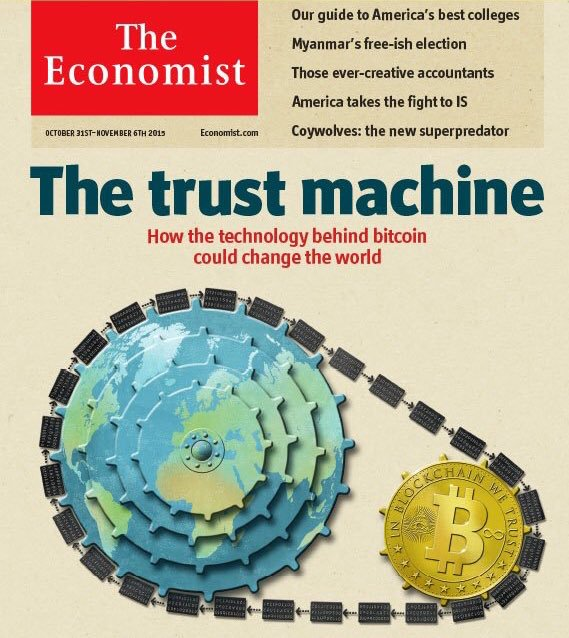
\includegraphics[height=6cm]{../pics/blockchain/economist-trust-machine}
	\end{figure}
}

\frame{
	\frametitle{But how does it work?}
	\begin{figure}
		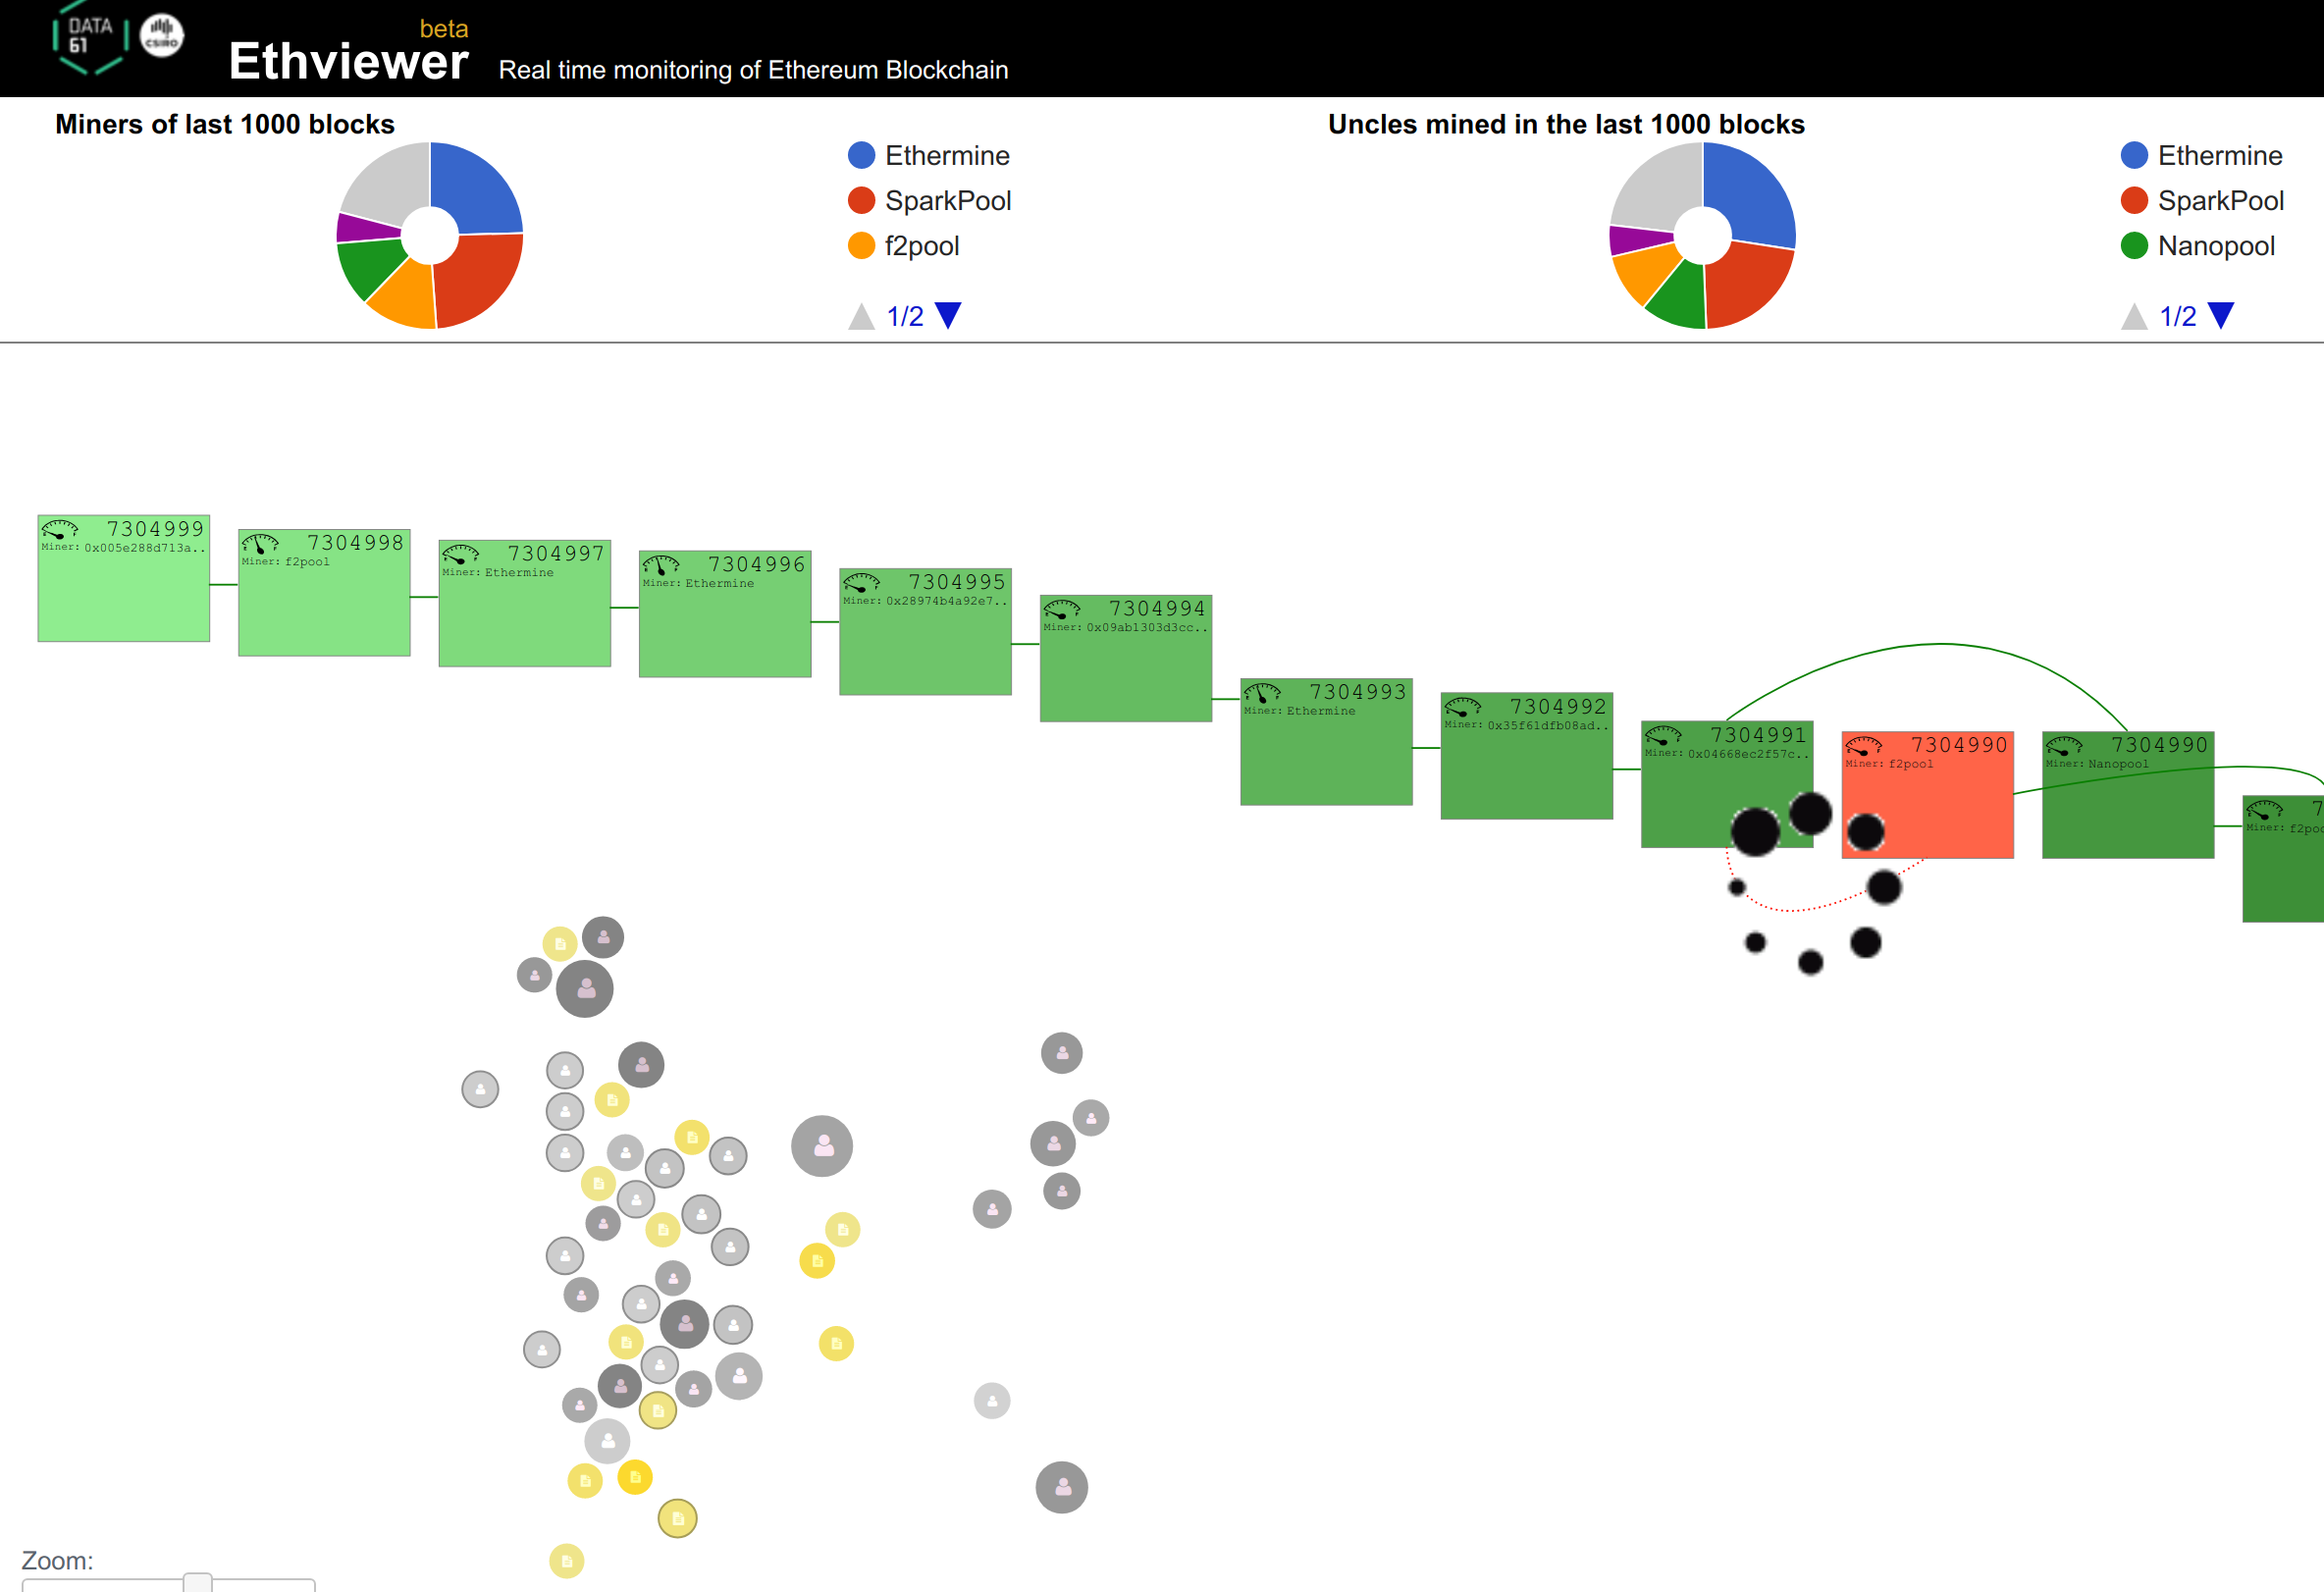
\includegraphics[height=6cm]{../pics/ethereum/ethviewer}
		\captionsetup{justification=centering}
		\caption{Source~: \url{http://ethviewer.live}}
	\end{figure}
}

\frame{
	\frametitle{Reference books}
	\framesubtitle{Blockchain in practice}
	\begin{columns}[T]
	\column{0.5\textwidth}
		\begin{figure}
			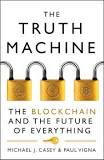
\includegraphics[height=4cm]{../pics/books/book-casey-truth.jpeg}
			\captionsetup{justification=centering}
			\caption{Book from \cite{casey2018:truth}}
		\end{figure}
	\column{0.5\textwidth}
		\begin{figure}
			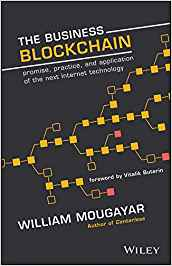
\includegraphics[height=4cm]{../pics/books/book-mougayar-business}
			\captionsetup{justification=centering}
			\caption{Book from \cite{mougayar:business}}
		\end{figure}
	\end{columns}
}

\frame{
	\frametitle{Ultimate references}
	The must-read white paper from legendary Satoshi Nakamoto: \textit{Bitcoin: A Peer-to-Peer Electronic Cash System} (\citeyear{satoshi:bitcoin-paper}),\\
	\vspace{1em}
	the Ethereum white paper from home-town Toronto Vitalik Buterin: \textit{A Next-Generation Smart Contract and Decentralized Application Platform} (\citeyear{buterin:ethereum-paper}),\\
	\vspace{1em}
	and the yellow paper authored by Prof. Gavin Wood: \textit{Ethereum: A secure decentralised generalised transaction ledger} (\citeyear{wood:ethereum-yellow-paper}).
}

% ======================================================================================================
%                         Tokens 
% ======================================================================================================
\section{Tokens Hands-On}
\frame{
	\frametitle{Create your own (ERC-20) token}
	\begin{figure}
		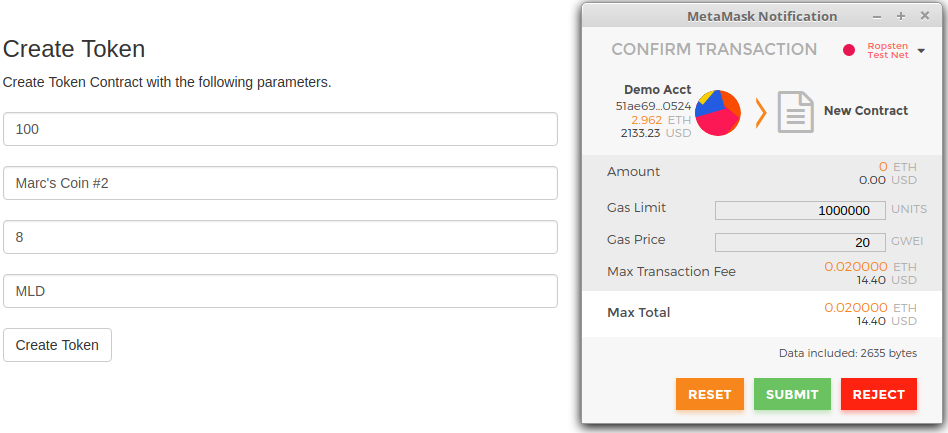
\includegraphics[width=10cm]{../pics/ethereum/token-factory-create}
	\end{figure}
	\vspace{-1em}
	\begin{enumerate}
		\item Use the Token Factory Dapp at \url{https://tokenfactory.surge.sh/\#/factory}
		\item MetaMask will pop up (see picture above)
		\item Submit the transaction (on the Ropsten Testnet)
		\item Check your transaction on \url{https://ropsten.etherscan.io} 
	\end{enumerate}
}

\frame{
	\frametitle{Check your Smart Contract}
	\begin{figure}
		
\includegraphics[width=10cm]{../pics/ethereum/metamask-contract-published}
	\end{figure}
	\vspace{-1em}
	\begin{enumerate}
		\item Select the ``Sent'' tab
		\item Check the orange Copy icon (Tx Hash) 
		\item Click on ``Contract Published''
		\item That should bring you to Etherscan (see next page)
	\end{enumerate}
}

\frame{
	\frametitle{Verify the status of your transaction on Etherscan}
	\begin{figure}
		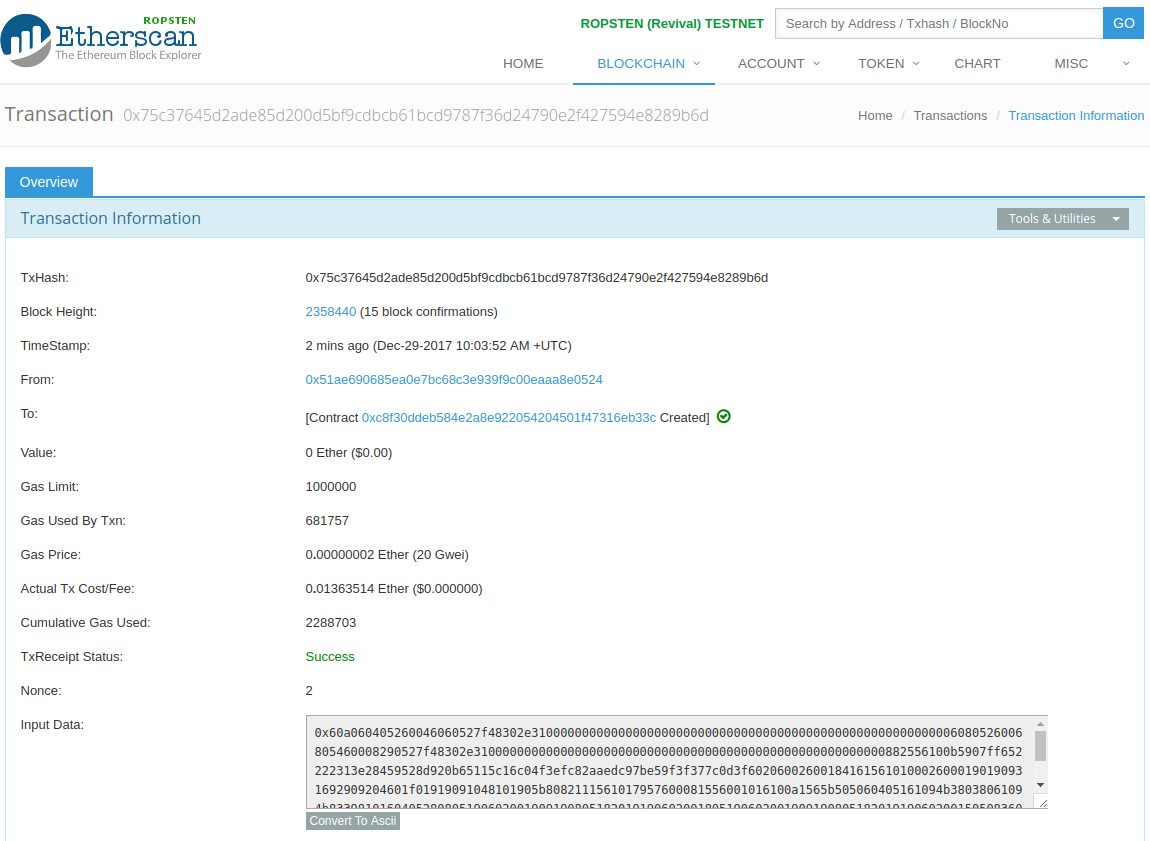
\includegraphics[width=10cm]{../pics/ethereum/etherscan-contract}
		\captionsetup{justification=centering}
		\caption*{Transaction Information: note the ``To'' line with your contract address}
	\end{figure}
}

\frame{
	\frametitle{Watch your Token}
	\begin{columns}
	\column{0.5\textwidth}
		\begin{figure}
			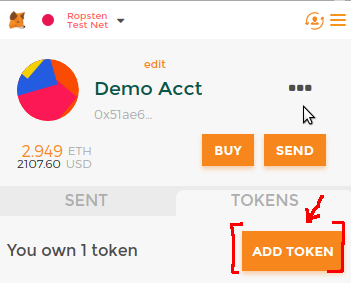
\includegraphics[width=3cm]{../pics/ethereum/metamask-add-token-1}
		\end{figure}
	\column{0.5\textwidth}
		\begin{figure}
			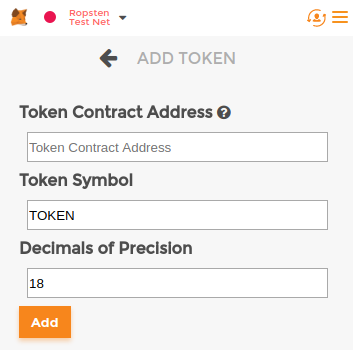
\includegraphics[width=3cm]{../pics/ethereum/metamask-add-token-2}
		\end{figure}
	\end{columns}
	\begin{enumerate}
		\item Click on the ``Add Token'' button
		\item Wait for the next window (picture on the right)
		\item Copy your contract address (from Etherscan)
		\item Go back to your Token Factory tab, which should show an UI to interact with your contract or go to the URL: https://tokenfactory.surge.sh/\#/token/0x... (replace 0x... by your contract address)
		\item Move coins around
		\item In MetaMask, click on your token to check the tx on Etherscan 
	\end{enumerate}
}

\frame{
	\frametitle{Most tokens are created this way}
	\begin{itemize}
		\item More than 50\% of the top~100 coins by market cap $^{\text{(*)}}$
		\item In 2018, it was 94\% according to ConsenSys
	\end{itemize}
	\vspace{1em}
	$^{\text{(*)}}$ \footnotesize{\emph{estimated April 2019 by cross-referencing the list of top ERC20 tokens by market cap on \href{https://eidoo.io/erc20-tokens-list/}{eidoo} and the list of all tokens by market cap on \href{https://cryptoli.st}{CryptoList}}}
}

\frame{
	\frametitle{Thousands of tokens in circulation}
	\begin{figure}
		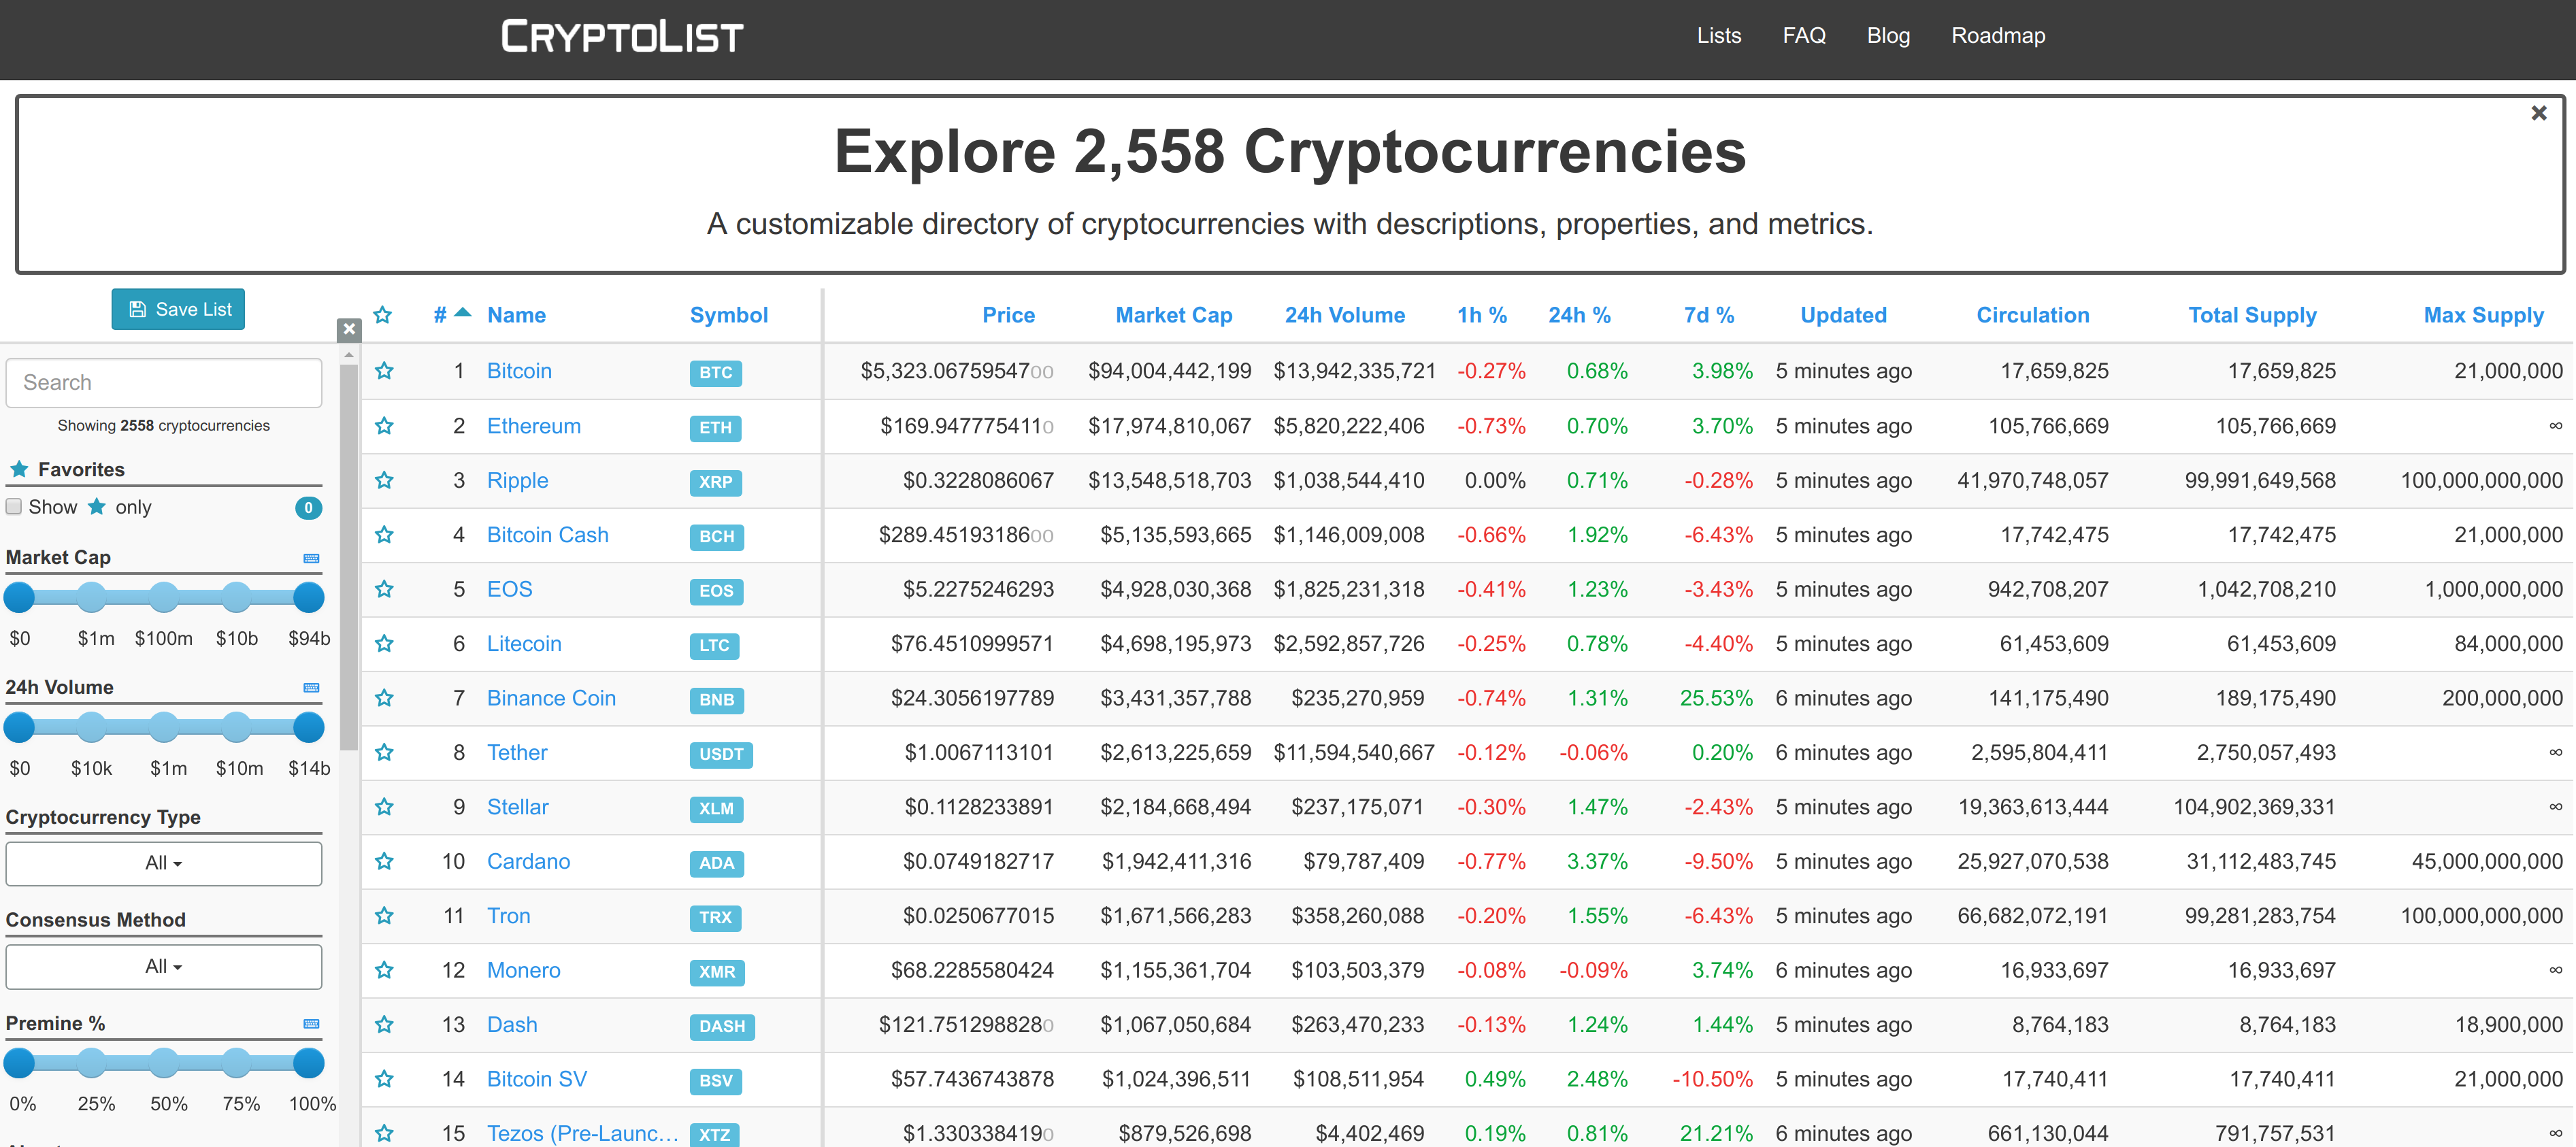
\includegraphics[width=11cm]{../pics/cryptocurrency/cryptolist-en}
		\captionsetup{justification=centering}
		\caption{Source~: \url{https://cryptoli.st}}
	\end{figure}
}

\frame{
	\frametitle{Back to business}
	\center\Huge 
	Tokens are cheap to make,\\
	so what?
}			

\frame{
	\frametitle{Large Fundraising}
	\framesubtitle{Biggest ICOs (by amount raised) --Join us next month to learn more!}
	\begin{figure}
		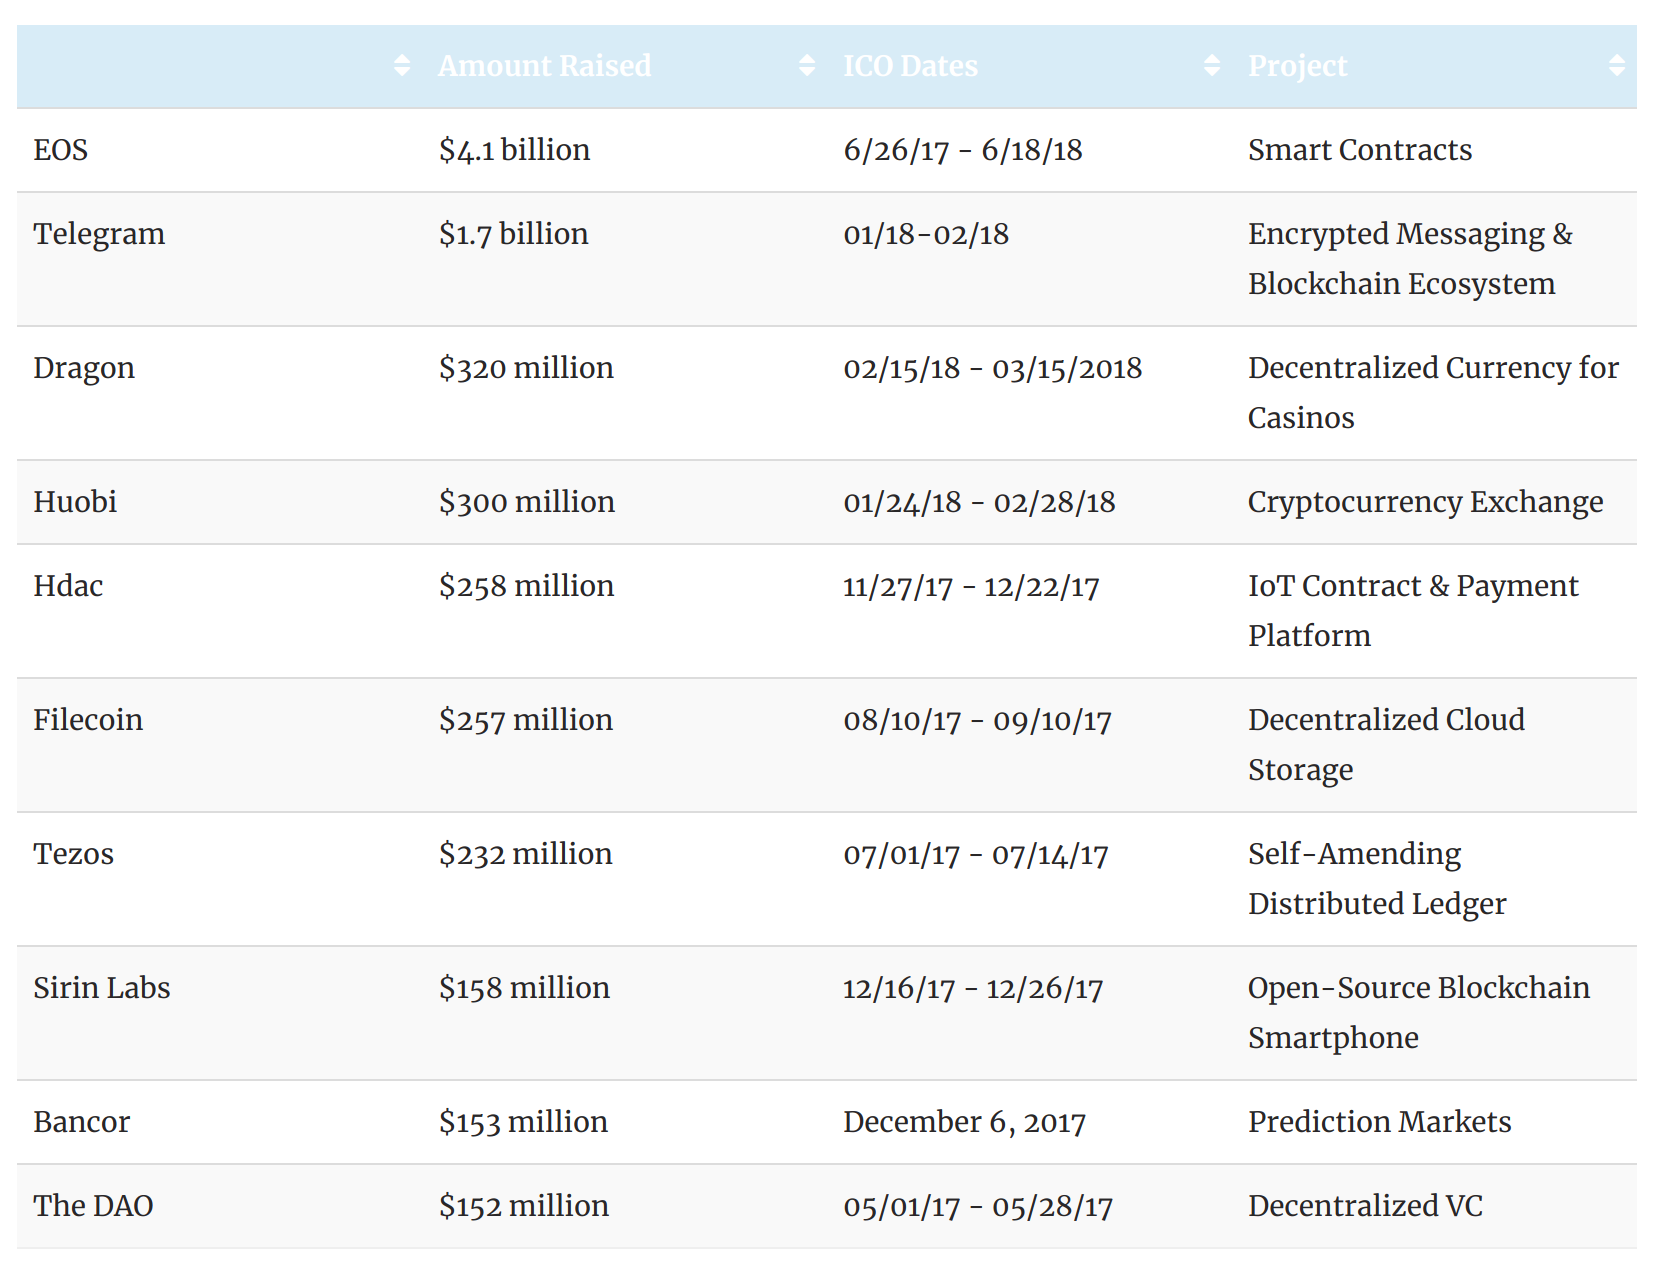
\includegraphics[height=6cm]{../pics/cryptocurrency/top10-icos-2018-short}
		\captionsetup{justification=centering}
		\caption{Source~: \cite{bicoinmarket201808:top10-ico}}
	\end{figure}
}

\frame{
	\frametitle{Native Currency}
	\begin{figure}
		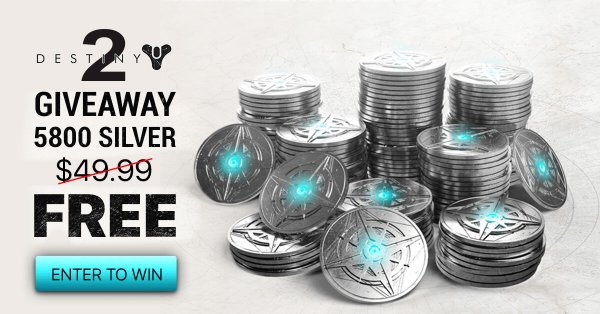
\includegraphics[height=6cm]{../pics/tokenization/destiny-silver}
		\captionsetup{justification=centering}
		\caption{Source~: give.zone (also sold on Amazon, PlayStation store, etc)}
	\end{figure}
}

\frame{
	\frametitle{A Token can represent anything}
	\begin{figure}
		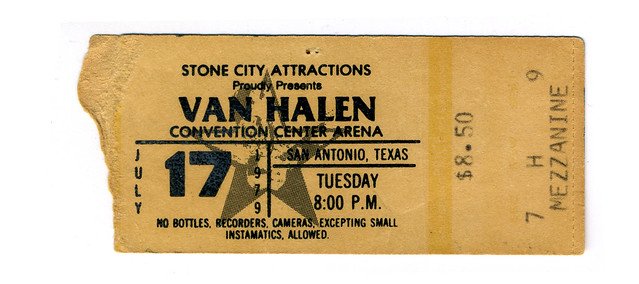
\includegraphics[width=11cm]{../pics/tokenization/ticket-van-halen}
		\captionsetup{justification=centering}
		\caption{Credit~: \href{https://www.flickr.com/photos/hmk/2121424630}{H. Michael Karshis}}
	\end{figure}
}


% ======================================================================================================
%                         Tokenization 
% ======================================================================================================
\section{Tokenization}
\frame{
	\frametitle{Case Study: Gold tokenization}
	\begin{figure}
		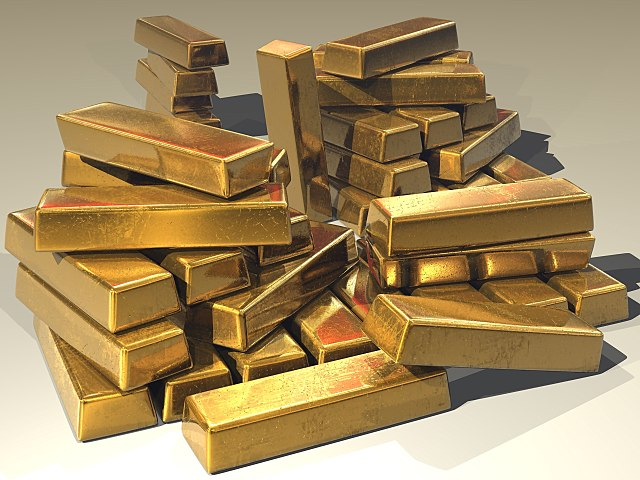
\includegraphics[height=3cm]{../pics/tokenization/640px-Gold_bullion_bars}
		\captionsetup{justification=centering}
		\caption{Credit~: \href{https://commons.wikimedia.org/wiki/File:Gold_bullion_bars.jpg}{stevebidmead}}
	\end{figure}
	\begin{itemize}
		\item JP Morgan tokenizes Gold (\cite{thetokenist2019:jpmorgangold})
		\item LAToken partners with MyGold (\cite{latoken2017:gold})
		\item \ldots 
	\end{itemize}
}

\frame{
	\frametitle{Case Studies: fractional real estate and track \& trace (Tuna)}
	\begin{figure}
		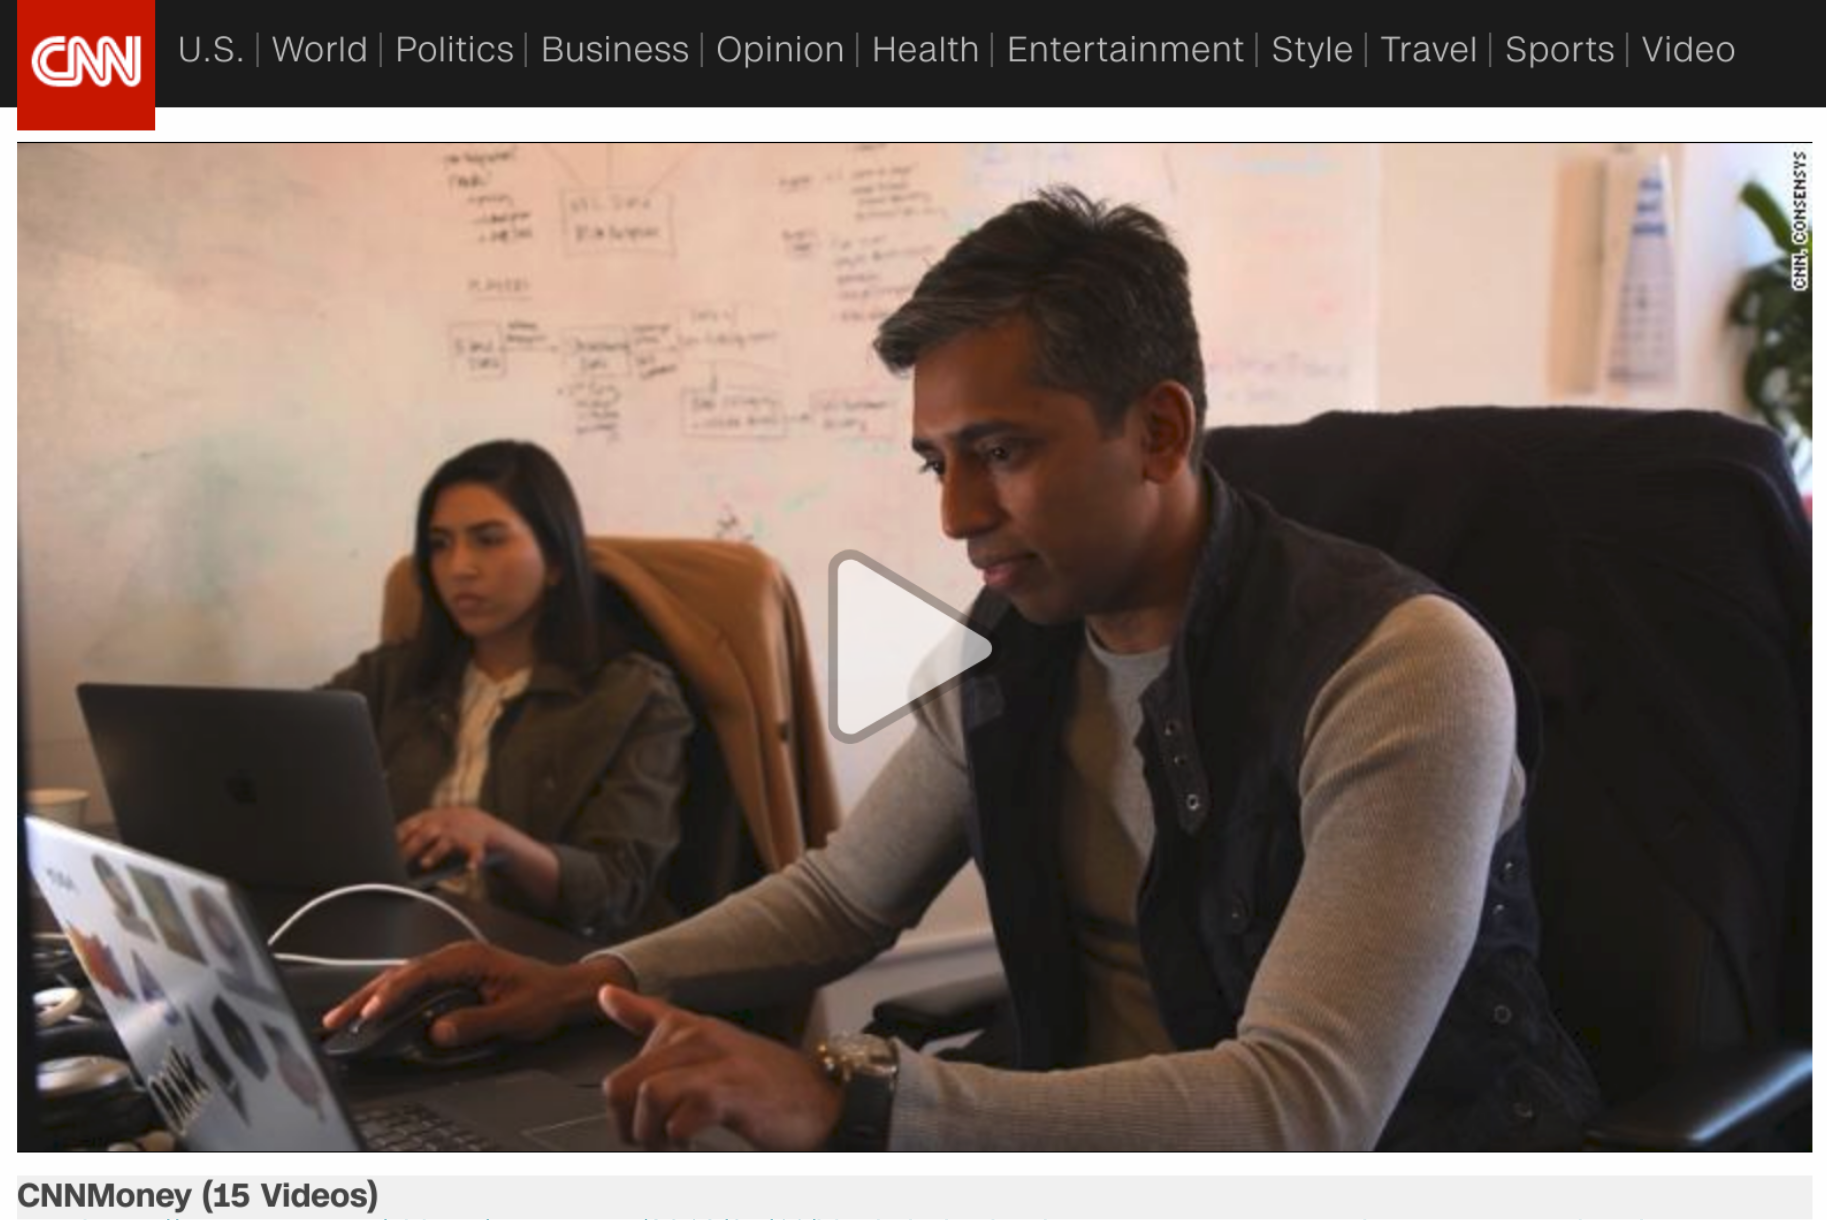
\includegraphics[height=6cm]{../pics/ConsenSys/case_studies/cnn2018-viant-meridio}
		\captionsetup{justification=centering}
		\caption{Source~: \cite{cnn2018:viant-meridio}}
	\end{figure}
}

\frame{
	\frametitle{Case Study: Ontario farmers sell corn on Blockchain rails}
	\framesubtitle{\tiny\url{https://farmtario.com/crops/ontario-farmers-make-first-blockchain-system-corn-sale/}}
	\begin{figure}
	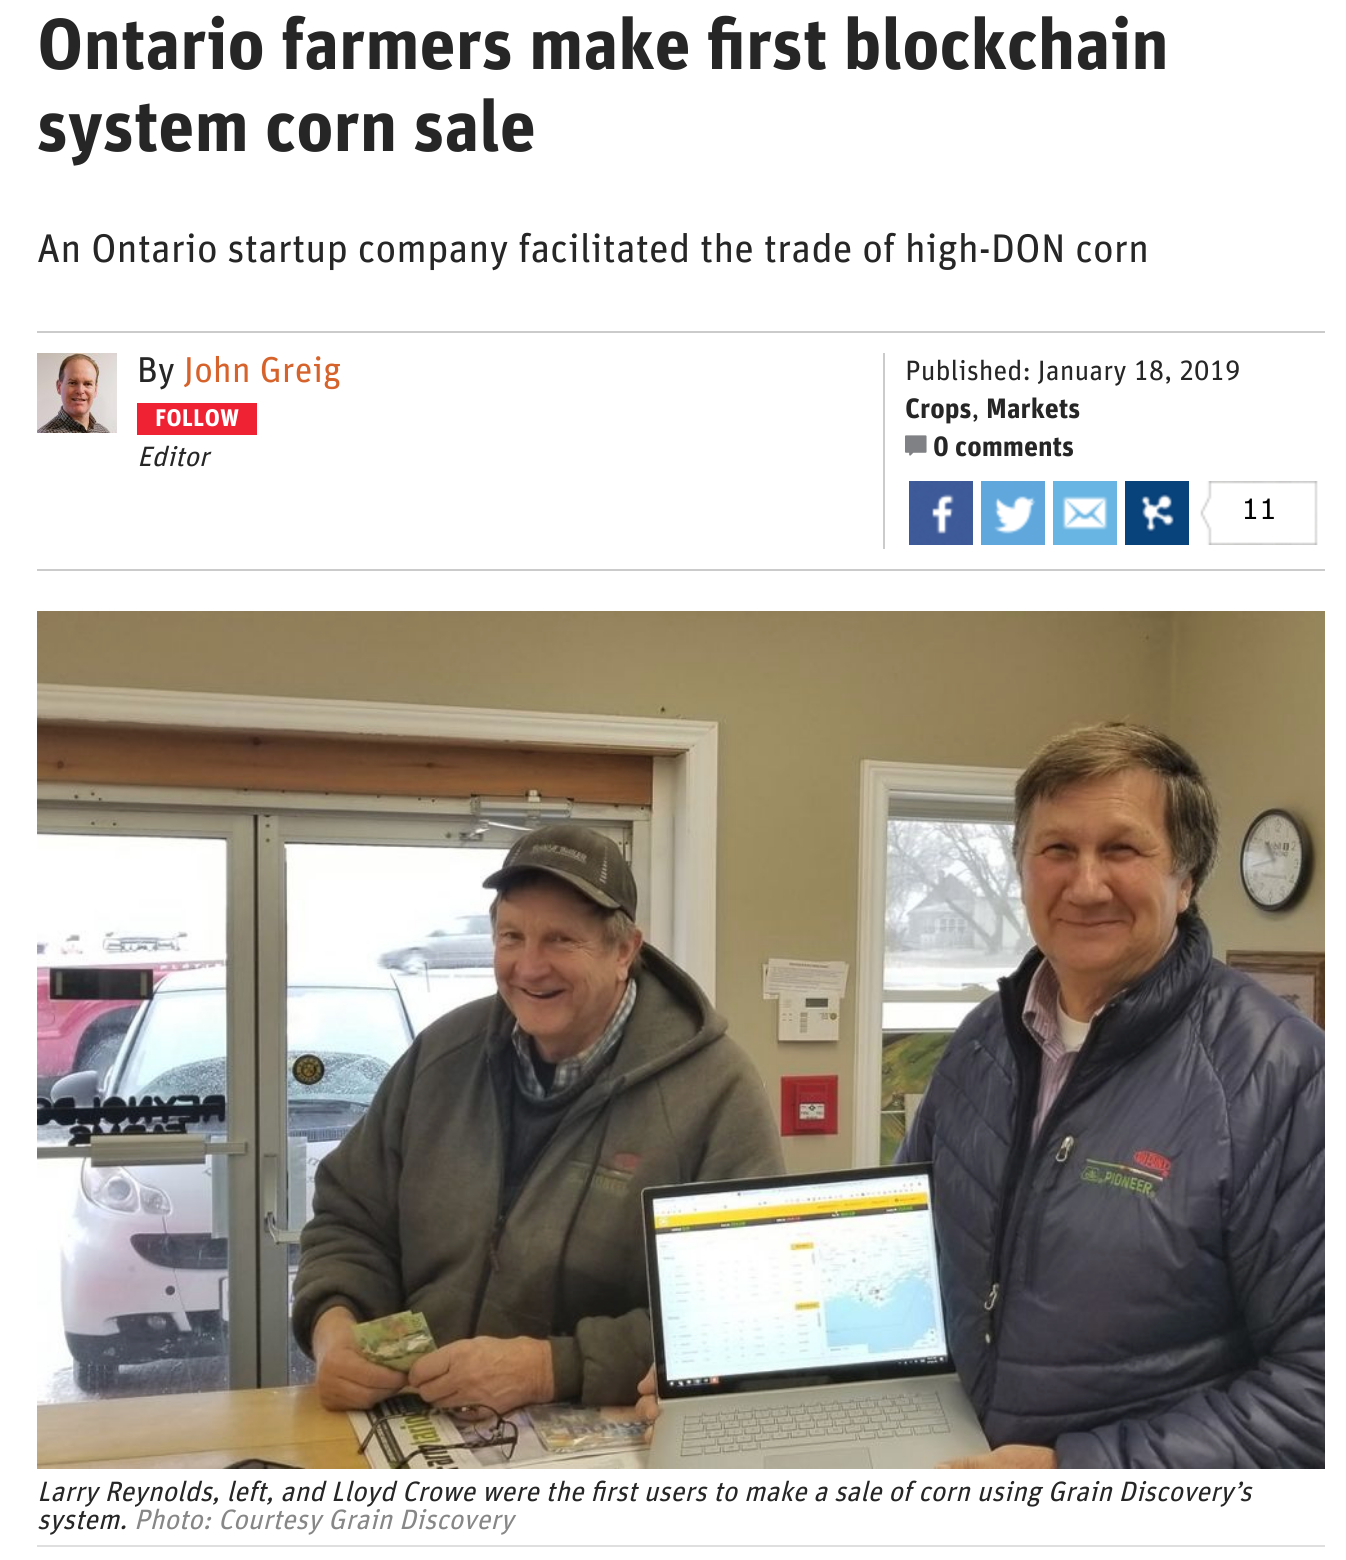
\includegraphics[height=6cm]{../pics/case_studies/ontario-farmers-corn2019}
	\end{figure}
}

\frame{
	\frametitle{Case Study: Walmart, Nestle, Unilever and others track the food supply chain}
	\framesubtitle{\tiny\url{https://cointelegraph.com/news/walmart-ibm-blockchain-initiative-aims-to-track-global-food-supply-chain}}
	\begin{figure}
	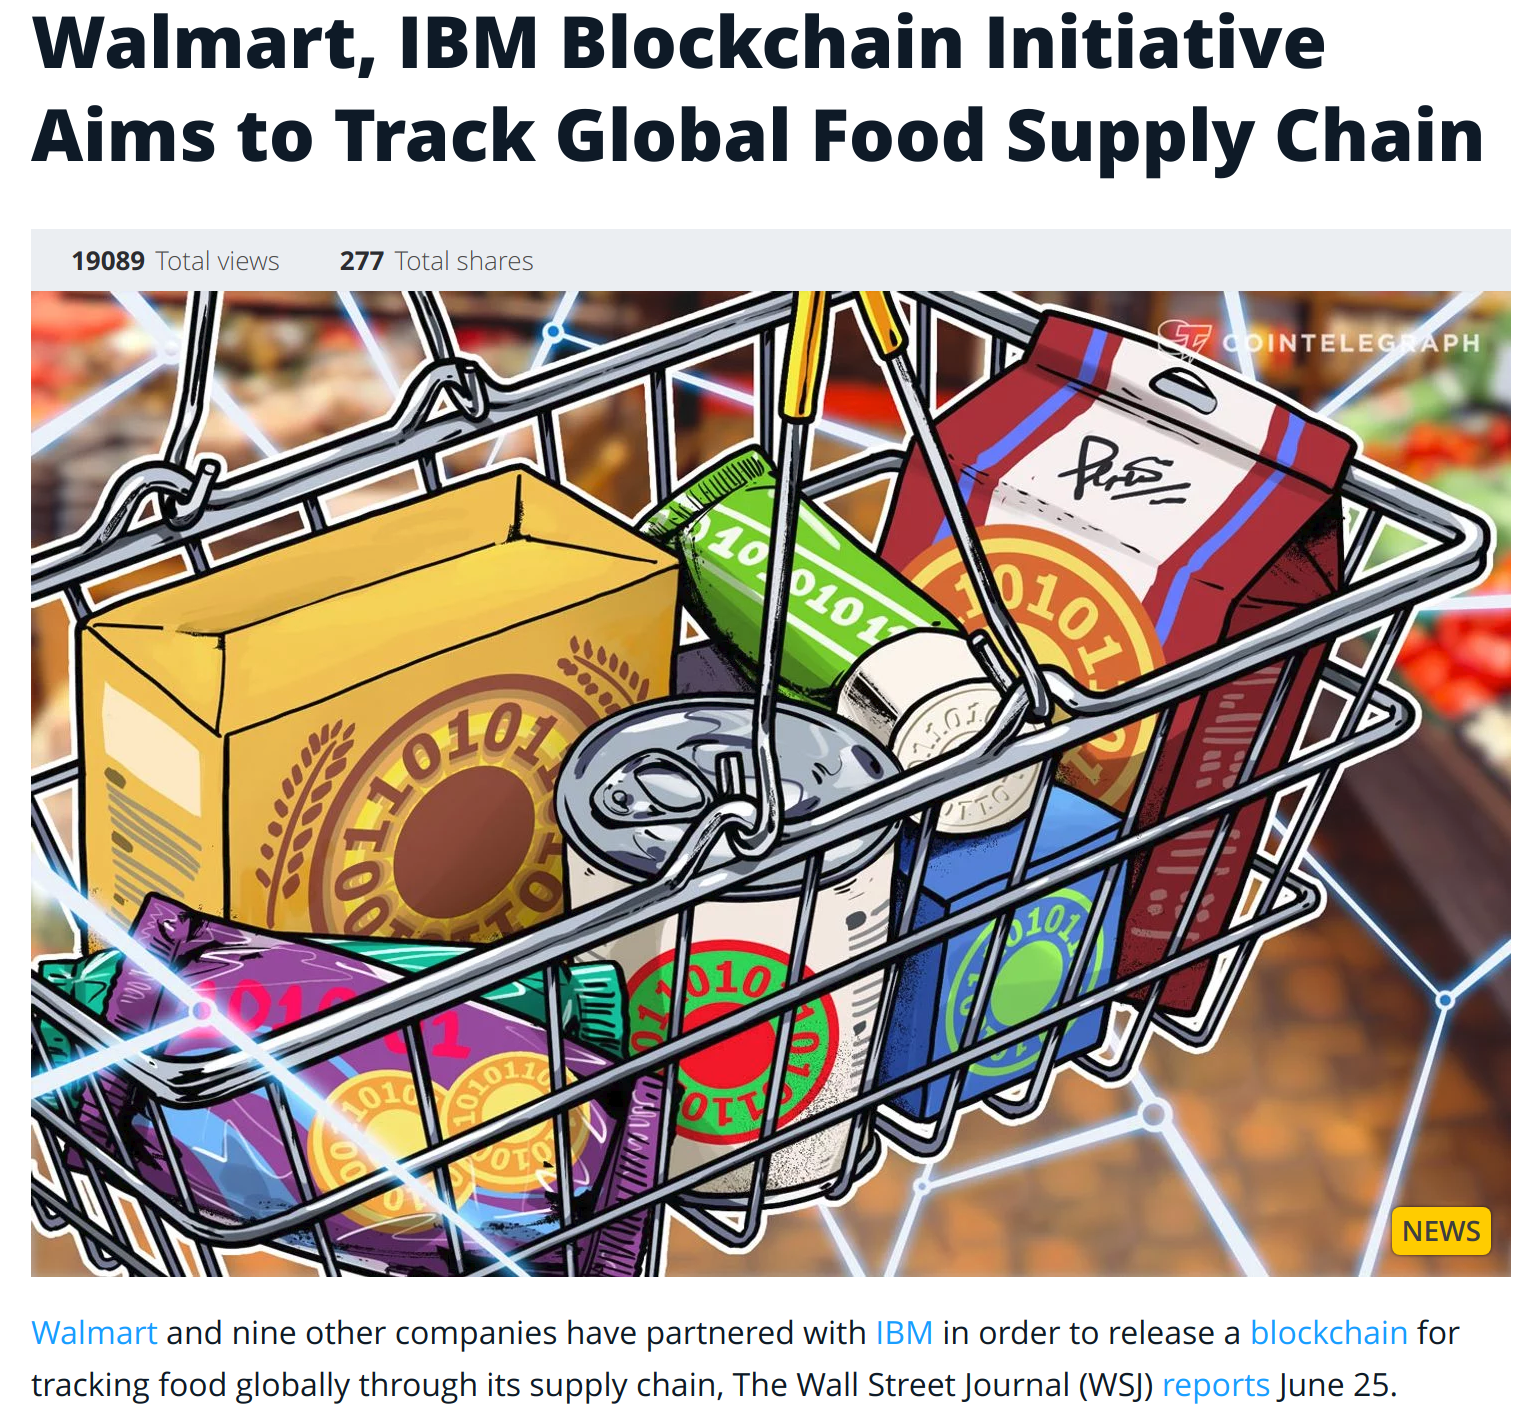
\includegraphics[height=6cm]{../pics/case_studies/walmart-ibm-2018}
	\end{figure}
}

\frame{
	\frametitle{Case Study: Trade Finance}
	%\framesubtitle{}
	\begin{figure}
	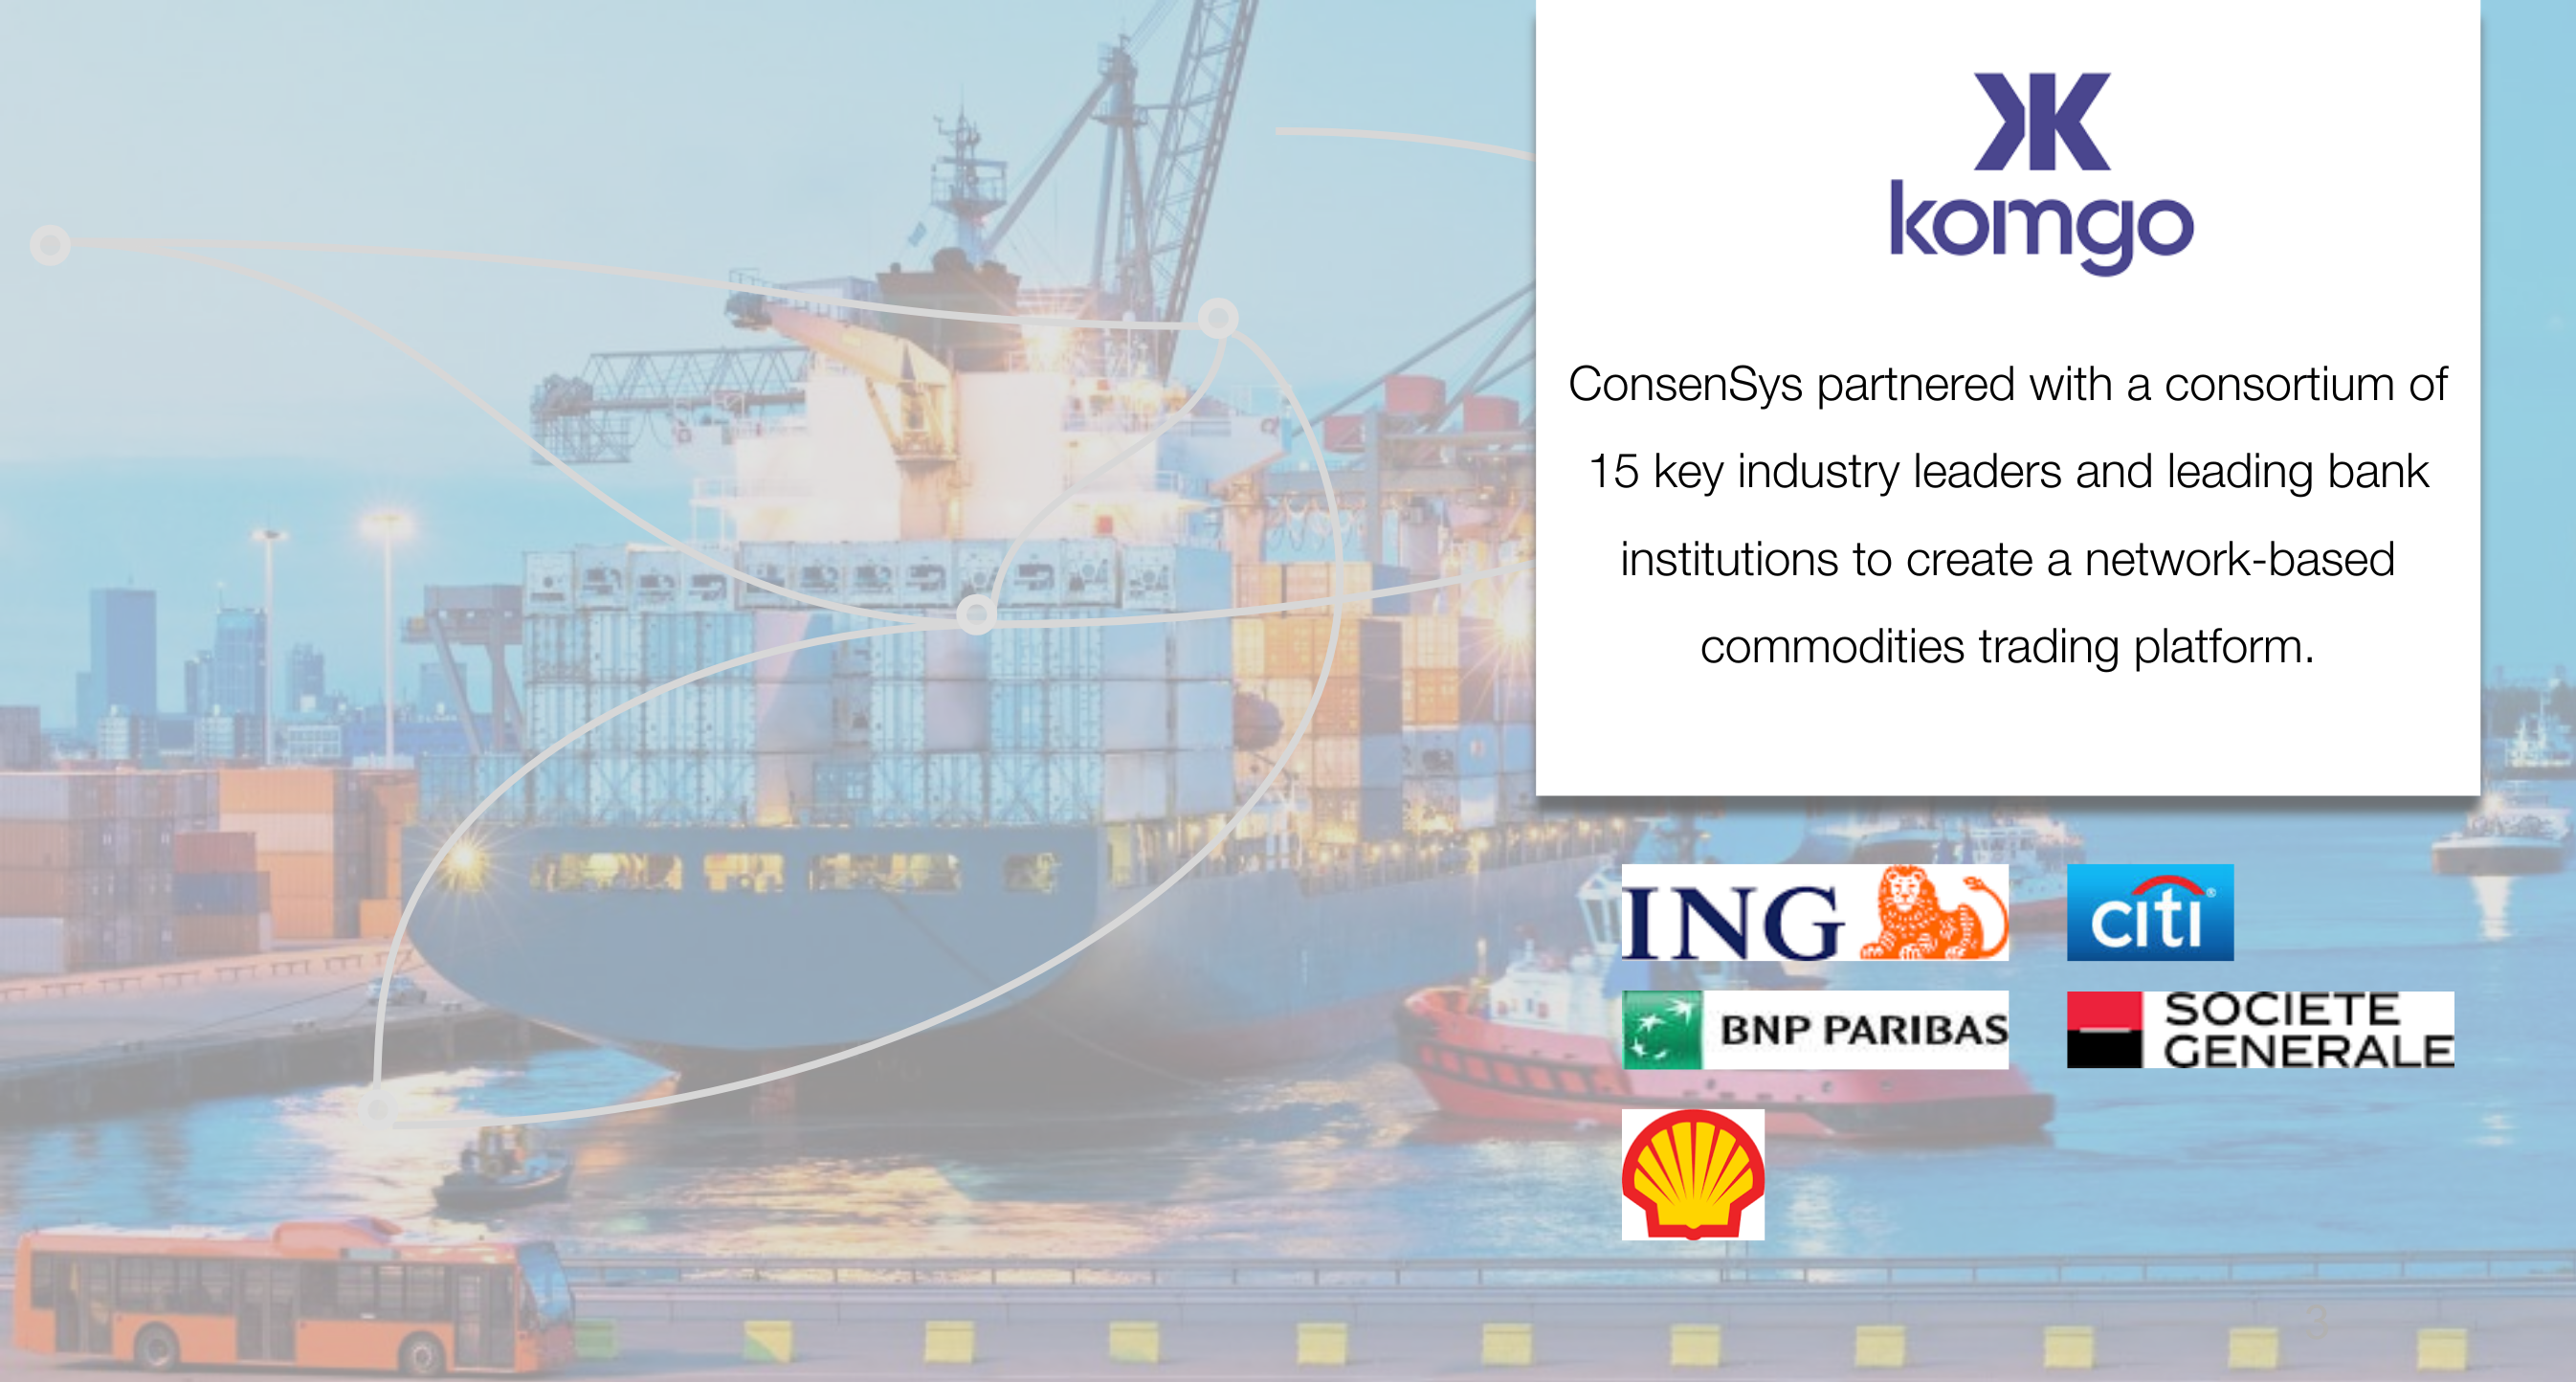
\includegraphics[height=6cm]{../pics/ConsenSys/case_studies/komgo}
	\end{figure}
}

\frame{
	\frametitle{Tokenization scenarios}	
	\begin{figure}
		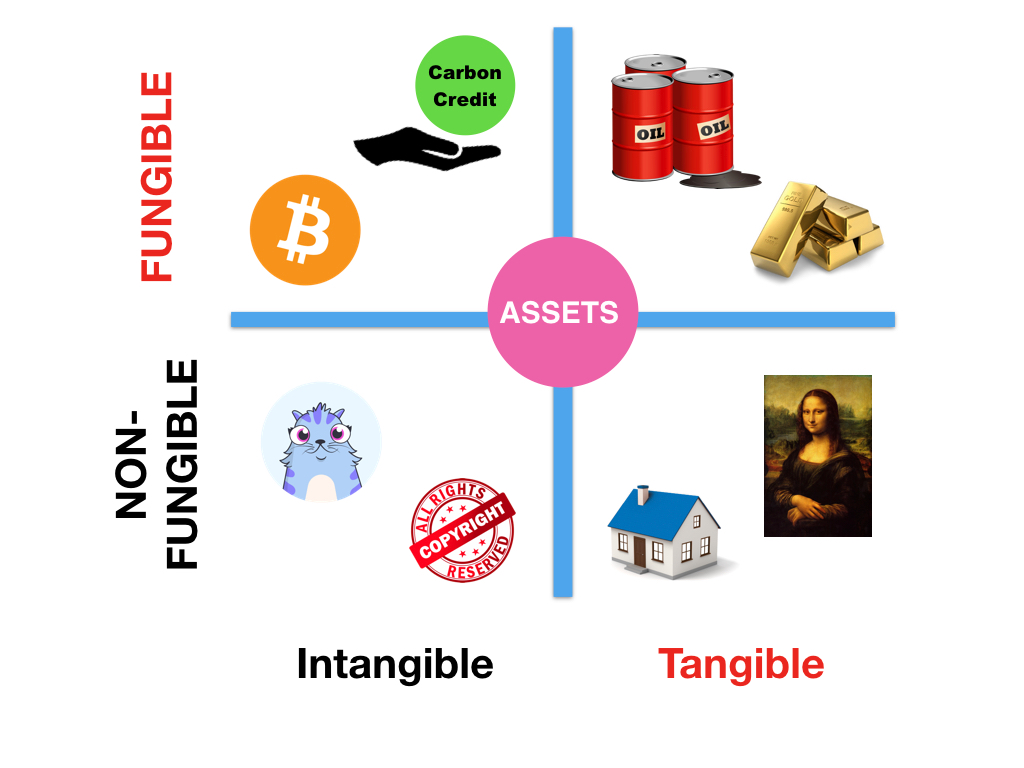
\includegraphics[height=7cm]{../pics/tokenization/fungible-vs-non-fungible}
		\captionsetup{justification=centering}
		\caption{Source~: \href{https://coindoo.com/fungible-vs-non-fungible-tokens-whats-the-difference/fungible-vs-non-fungible/}{Coindoo}}
	\end{figure}
}

\frame{
	\frametitle{What did we learn?}
	\center\Huge 
	Tokenization is a mechanism to manage and trade\\
	anything \emph{digitally}\\
	with the same trust and benefits (or more) as with Bitcoin.
}			


% ======================================================================================================
%                         Token Economy 
% ======================================================================================================
\section{Token Economy}
\frame{
	\frametitle{What's an Economy?}
%	\begin{quote}
%		An economy (from Greek oikos % need UTF8 to render this in greek: \textomikron\textiota\textkappa\textomikron\textsigma %οίκος 
%		– "household" and νέμoμαι – "manage") is an area of the production, distribution, or trade, and consumption of goods and services by different agents. Understood in its broadest sense, 'The economy is defined as a social domain that emphasize the practices, discourses, and material expressions associated with the production, use, and management of resources'. Economic agents can be individuals, businesses, organizations, or governments. Economic transactions occur when two parties agree to the value or price of the transacted good or service, commonly expressed in a certain currency. However, monetary transactions only account for a small part of the economic domain.
%	\end{quote}
	\begin{figure}
		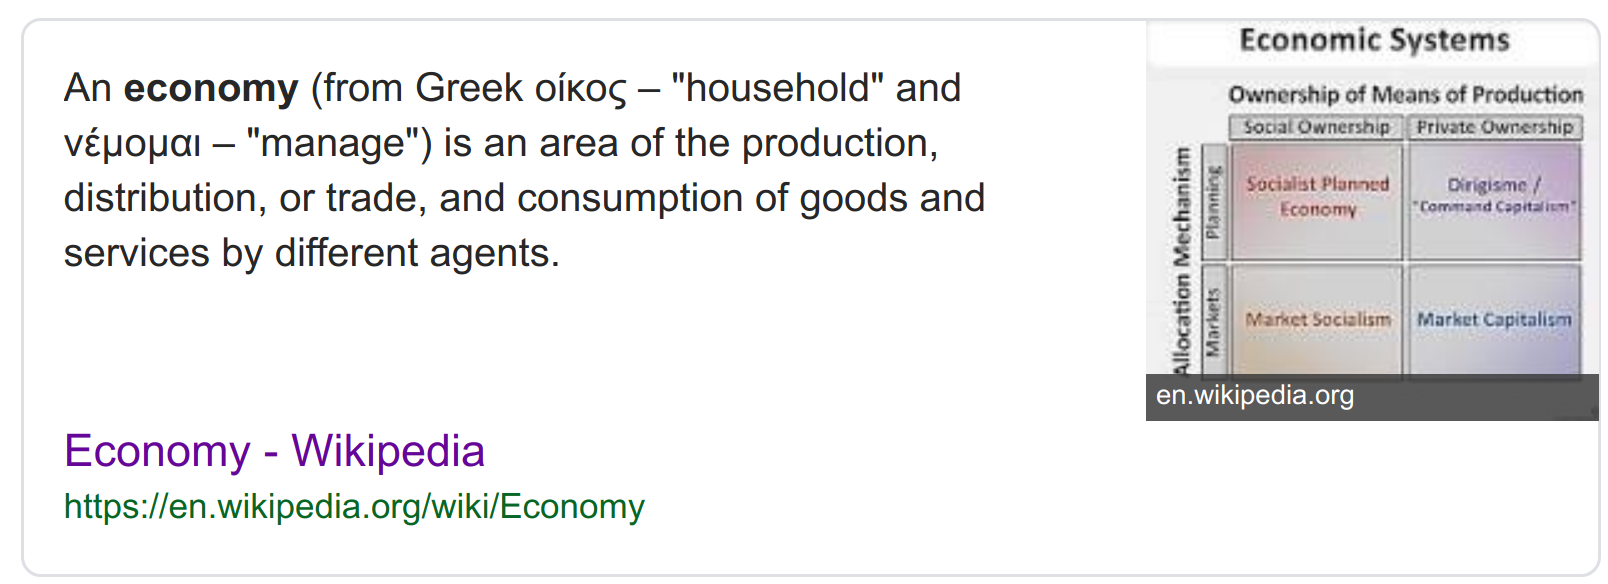
\includegraphics[width=11cm]{../pics/tokenization/economy-definition}
	\end{figure}
}

\frame{
	\frametitle{Economics 101}
	\begin{figure}
		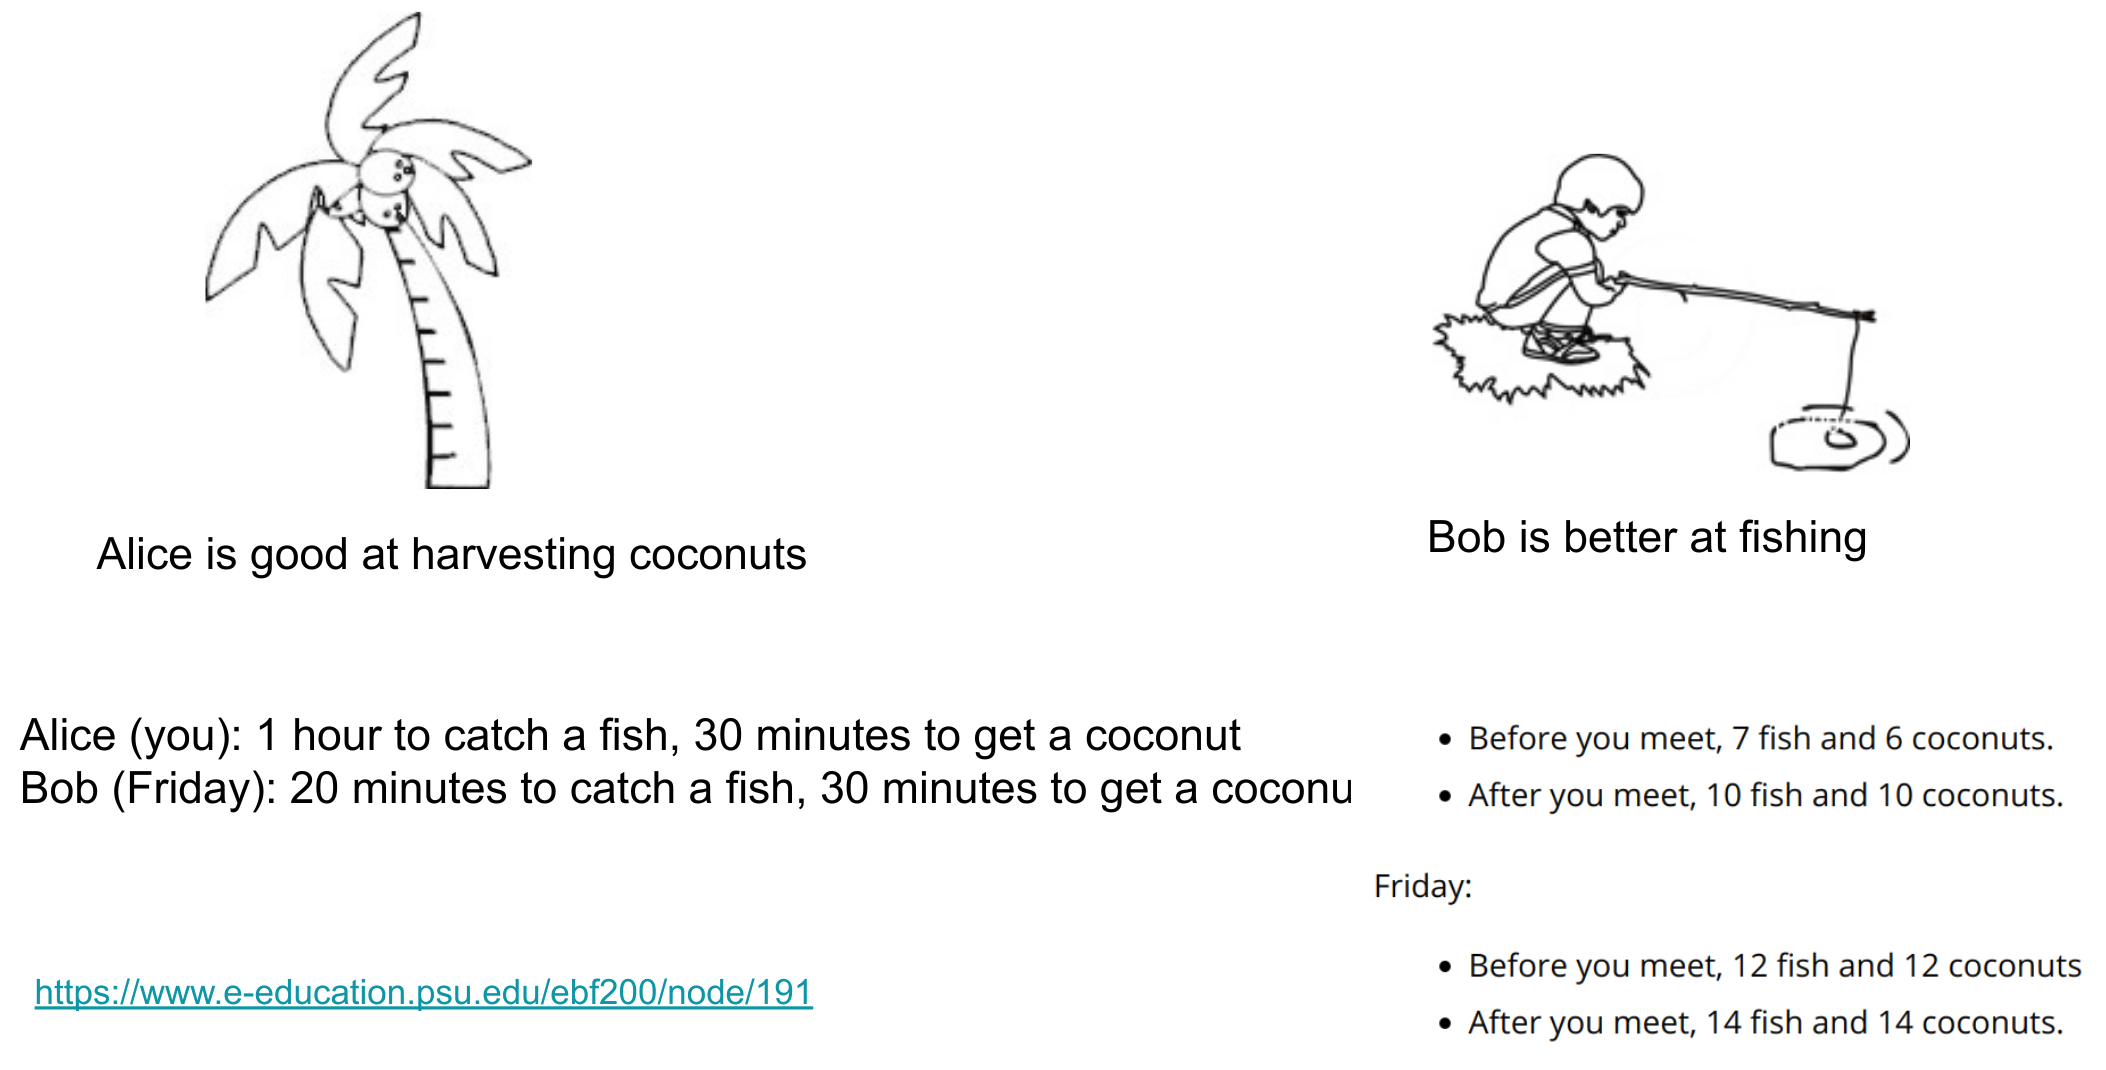
\includegraphics[width=11cm]{../pics/tokenization/economy-coconut-fish}
		\captionsetup{justification=centering}
		\caption{Source~: \cite{psuebf200}}
	\end{figure}
}

\frame{
	\frametitle{Contribution of Blockchain}
	\begin{itemize}
		\item Internet of value
		\item trust
		\item tamper-resistant
		\item auditable
		\item programmable!
		\item \ldots
	\end{itemize}
}

\frame{
	\frametitle{Automated peer-to-peer compensation}	
	\begin{figure}
		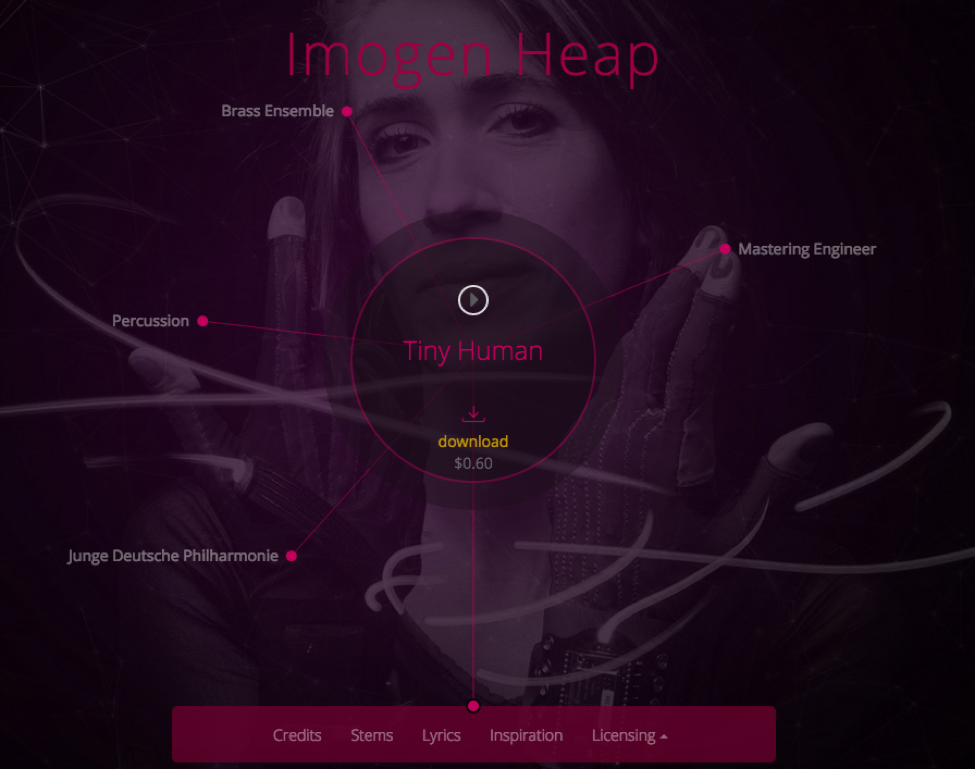
\includegraphics[height=7cm]{../pics/tokenization/ujomusic-heap}
		\captionsetup{justification=centering}
		\caption{Source~: \href{https://media.consensys.net/evolution-of-ujo-music-the-tiny-human-retrospective-e23136197c31}{Ujo Music}}
	\end{figure}
}

\frame{
	\frametitle{In Toronto: Prescient is developing an Attribution Ledger for Work of Arts}	
	\begin{figure}
		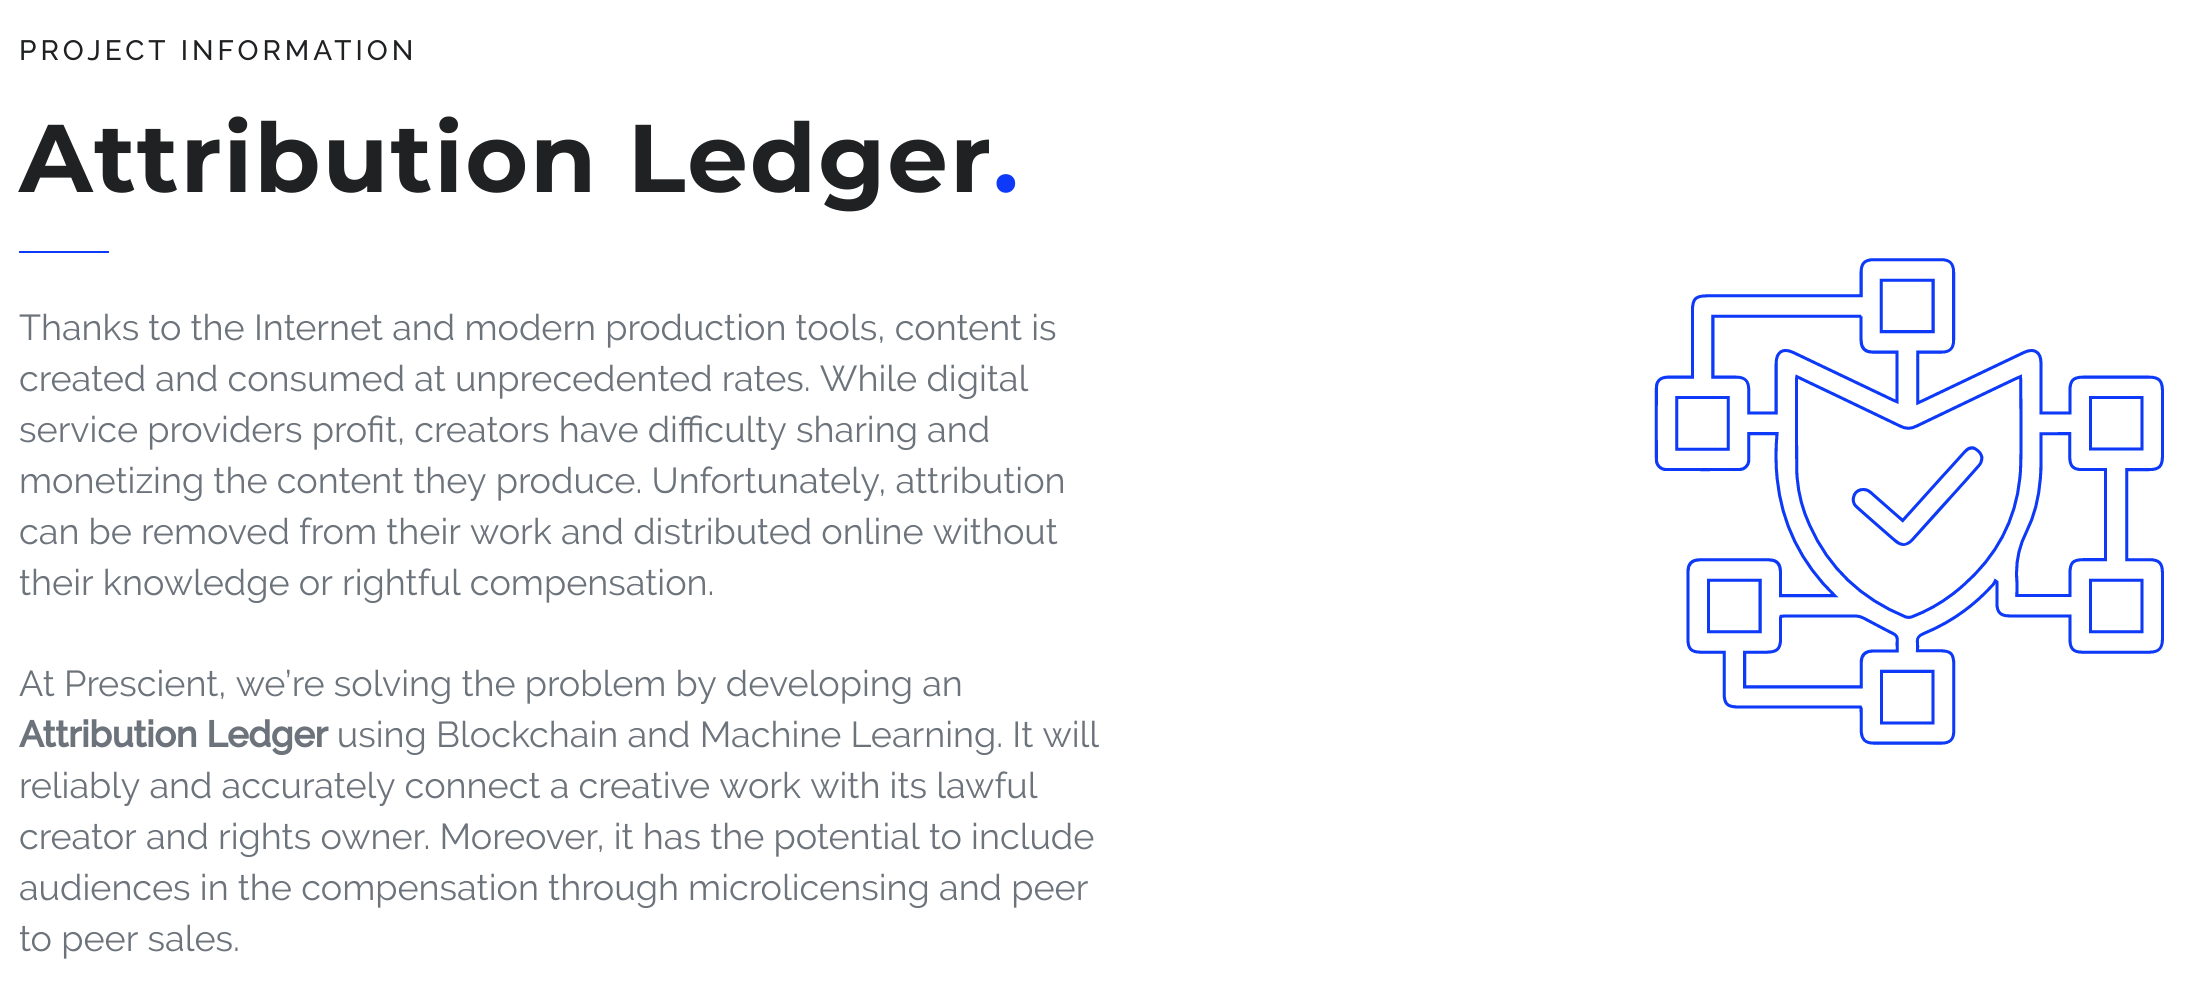
\includegraphics[width=11cm]{../pics/tokenization/prescient-attribution-ledger}
		\captionsetup{justification=centering}
		\caption{Source~: \url{https://prescientinnovations.com/attribution-ledger}}
	\end{figure}
}

\frame{
	\frametitle{The "free" economy}	
	\begin{figure}
		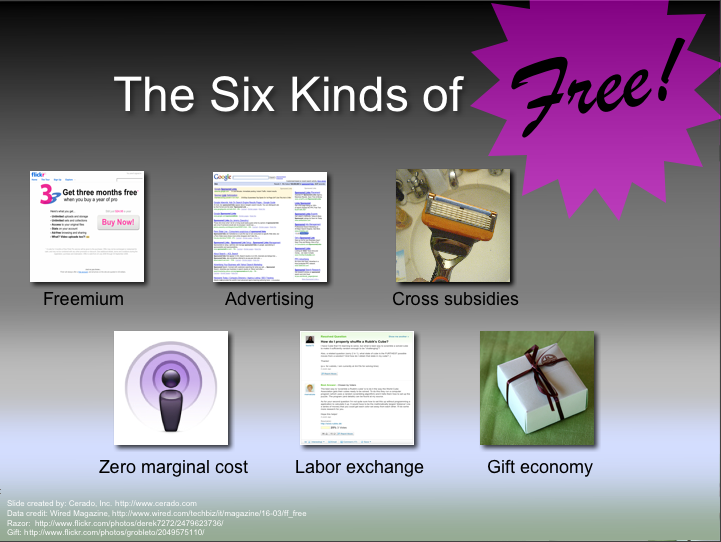
\includegraphics[height=7cm]{../pics/tokenization/six-kind-of-free}
		\captionsetup{justification=centering}
		\caption{Credit~: \href{https://www.flickr.com/photos/53341558@N00/2759517762}{Christopher Carfi}}
	\end{figure}
}

\frame{
	\frametitle{In Toronto: Midata is developing a platform to get paid for usage data while maintaining privacy}	
	\begin{figure}
		
\includegraphics[width=11cm]{../pics/tokenization/midata-clip}
		\captionsetup{justification=centering}
		\caption{Source~: \url{https://midata.io}}
	\end{figure}
}

\frame{
	\frametitle{The "sharing" economy}	
	\begin{figure}
		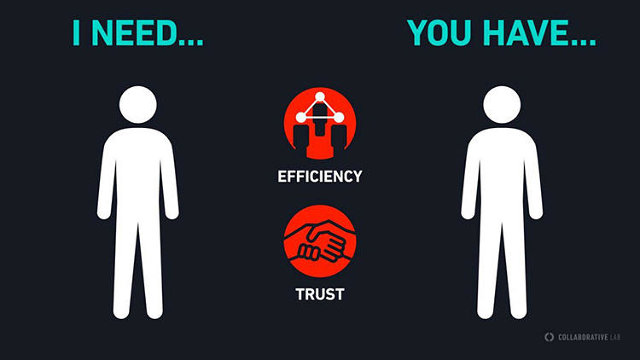
\includegraphics[width=11cm]{../pics/tokenization/sharing-economy-tira94}
		\captionsetup{justification=centering}
		\caption{Credit~: \href{https://hu.wikipedia.org/wiki/Wikip\%C3\%A9dia:Sharing_economy\#/media/File:3022028-inline-3022028-slide-slide-16-1024.jpg}{Tira94}}
	\end{figure}
}

\frame{
	\frametitle{Token-Curated Registries (TCRs)}
	\begin{figure}
		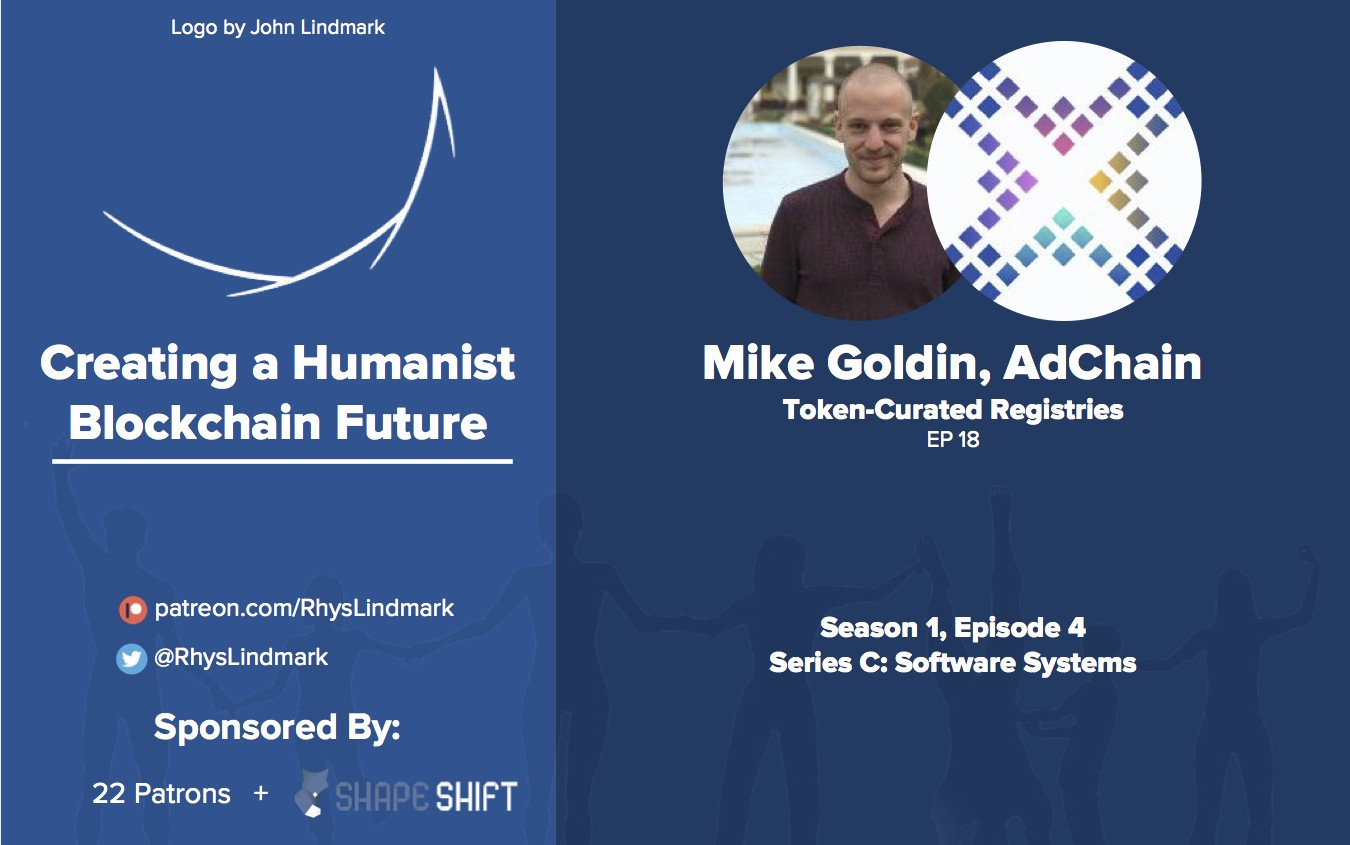
\includegraphics[width=11cm]{../pics/tokenization/goldin-podcast}
		\captionsetup{justification=centering}
		\caption{Source~: \cite{goldin2017:podcast}}
	\end{figure}
}

\frame{
	\frametitle{Token Economy approach from Outlier Ventures}
% https://outlierventures.io/wp-content/uploads/2018/10/Token-Ecosystem-Creation-Outlier-Ventures-PDF.pdf
	\begin{figure}
%		
\includegraphics[width=11cm]{../pics/tokenization/outlier-token-design}
		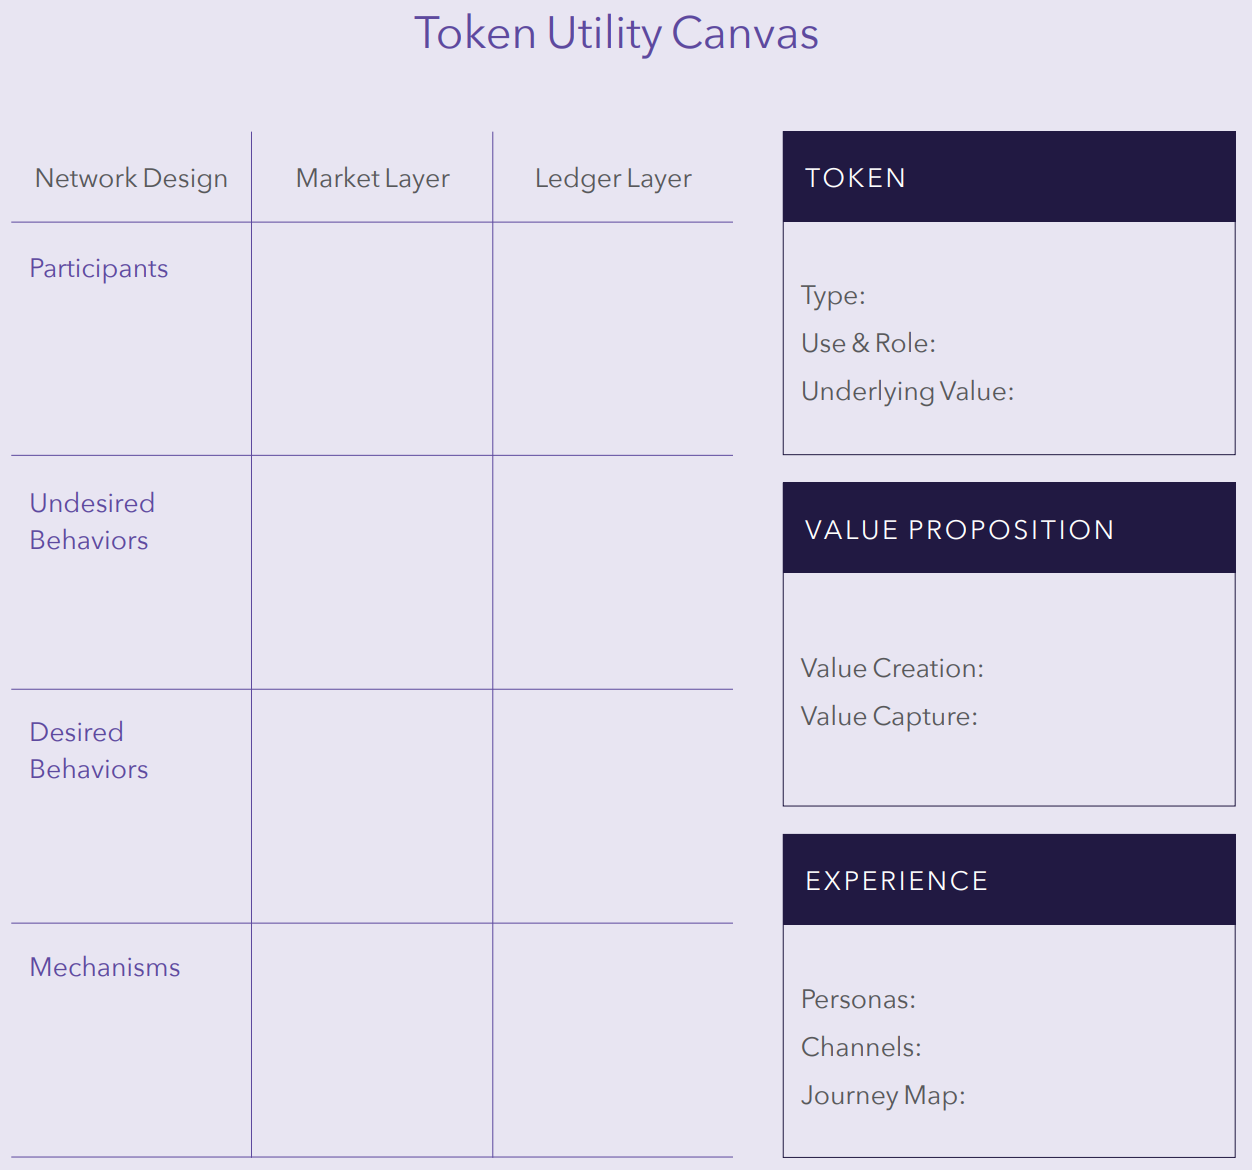
\includegraphics[height=7cm]{../pics/tokenization/outlier-ventures-token-utility-canvas}
		\captionsetup{justification=centering}
		\caption{Source~: \cite{outlier:tokenisation}}
	\end{figure}
}




